\batchmode
\documentclass[twoside]{book}

% Packages required by doxygen
\usepackage{fixltx2e}
\usepackage{calc}
\usepackage{doxygen}
\usepackage[export]{adjustbox} % also loads graphicx
\usepackage{graphicx}
\usepackage[utf8]{inputenc}
\usepackage{makeidx}
\usepackage{multicol}
\usepackage{multirow}
\PassOptionsToPackage{warn}{textcomp}
\usepackage{textcomp}
\usepackage[nointegrals]{wasysym}
\usepackage[table]{xcolor}

% Font selection
\usepackage[T1]{fontenc}
\usepackage[scaled=.90]{helvet}
\usepackage{courier}
\usepackage{amssymb}
\usepackage{sectsty}
\renewcommand{\familydefault}{\sfdefault}
\allsectionsfont{%
  \fontseries{bc}\selectfont%
  \color{darkgray}%
}
\renewcommand{\DoxyLabelFont}{%
  \fontseries{bc}\selectfont%
  \color{darkgray}%
}
\newcommand{\+}{\discretionary{\mbox{\scriptsize$\hookleftarrow$}}{}{}}

% Page & text layout
\usepackage{geometry}
\geometry{%
  a4paper,%
  top=2.5cm,%
  bottom=2.5cm,%
  left=2.5cm,%
  right=2.5cm%
}
\tolerance=750
\hfuzz=15pt
\hbadness=750
\setlength{\emergencystretch}{15pt}
\setlength{\parindent}{0cm}
\setlength{\parskip}{3ex plus 2ex minus 2ex}
\makeatletter
\renewcommand{\paragraph}{%
  \@startsection{paragraph}{4}{0ex}{-1.0ex}{1.0ex}{%
    \normalfont\normalsize\bfseries\SS@parafont%
  }%
}
\renewcommand{\subparagraph}{%
  \@startsection{subparagraph}{5}{0ex}{-1.0ex}{1.0ex}{%
    \normalfont\normalsize\bfseries\SS@subparafont%
  }%
}
\makeatother

% Headers & footers
\usepackage{fancyhdr}
\pagestyle{fancyplain}
\fancyhead[LE]{\fancyplain{}{\bfseries\thepage}}
\fancyhead[CE]{\fancyplain{}{}}
\fancyhead[RE]{\fancyplain{}{\bfseries\leftmark}}
\fancyhead[LO]{\fancyplain{}{\bfseries\rightmark}}
\fancyhead[CO]{\fancyplain{}{}}
\fancyhead[RO]{\fancyplain{}{\bfseries\thepage}}
\fancyfoot[LE]{\fancyplain{}{}}
\fancyfoot[CE]{\fancyplain{}{}}
\fancyfoot[RE]{\fancyplain{}{\bfseries\scriptsize Generated by Doxygen }}
\fancyfoot[LO]{\fancyplain{}{\bfseries\scriptsize Generated by Doxygen }}
\fancyfoot[CO]{\fancyplain{}{}}
\fancyfoot[RO]{\fancyplain{}{}}
\renewcommand{\footrulewidth}{0.4pt}
\renewcommand{\chaptermark}[1]{%
  \markboth{#1}{}%
}
\renewcommand{\sectionmark}[1]{%
  \markright{\thesection\ #1}%
}

% Indices & bibliography
\usepackage{natbib}
\usepackage[titles]{tocloft}
\setcounter{tocdepth}{3}
\setcounter{secnumdepth}{5}
\makeindex

% Hyperlinks (required, but should be loaded last)
\usepackage{ifpdf}
\ifpdf
  \usepackage[pdftex,pagebackref=true]{hyperref}
\else
  \usepackage[ps2pdf,pagebackref=true]{hyperref}
\fi
\hypersetup{%
  colorlinks=true,%
  linkcolor=blue,%
  citecolor=blue,%
  unicode%
}

% Custom commands
\newcommand{\clearemptydoublepage}{%
  \newpage{\pagestyle{empty}\cleardoublepage}%
}

\usepackage{caption}
\captionsetup{labelsep=space,justification=centering,font={bf},singlelinecheck=off,skip=4pt,position=top}

%===== C O N T E N T S =====

\begin{document}

% Titlepage & ToC
\hypersetup{pageanchor=false,
             bookmarksnumbered=true,
             pdfencoding=unicode
            }
\pagenumbering{alph}
\pagenumbering{arabic}
\hypersetup{pageanchor=true}

%--- Begin generated contents ---
\chapter{Time-\/harmonic acoustic fluid-\/structure interaction problems}
\label{index}\hypertarget{index}{}\hypertarget{index_q}{}\section{A few quick questions...}\label{index_q}
Since {\ttfamily oomph-\/lib} is developed as open-\/source software, any evidence that the code is being downloaded and used is very helpful for us as it helps to justify our continued work on this project.

We would therefore be extremely grateful if you could provide the information requested in the form below. Pressing the \char`\"{}submit\char`\"{} button will get you to the actual download page.

{\bfseries Note\+:} 
\begin{DoxyItemize}
\item All information will be treated as confidential. 
\item If you provide your email address and check the appropriate box we will add you to our mailing list to inform you of upgrades and bug fixes to the code. Rest assured that the mailing list is {\bfseries very low volume} -- we have better things to do than to bombard you with email. 
\item If you still feel reluctant to provide any of the information requested, feel free to enter some dummy input. The form will check that {\bfseries some} information has been entered but entering your name as \char`\"{}\+Joe Cool\char`\"{} is perfectly acceptable -- this is to discourage people from not providing the information simply because they are too lazy to type... 
\end{DoxyItemize}



 







 

 \hypertarget{index_pdf}{}\section{P\+D\+F file}\label{index_pdf}
A \href{../latex/refman.pdf}{\tt pdf version} of this document is available. \end{document}

\chapter{Namespace Index}
\section{Namespace List}
Here is a list of all namespaces with brief descriptions\+:\begin{DoxyCompactList}
\item\contentsline{section}{\hyperlink{namespaceGlobal__Physical__Variables}{Global\+\_\+\+Physical\+\_\+\+Variables} \\*Global variables that represent physical properties }{\pageref{namespaceGlobal__Physical__Variables}}{}
\item\contentsline{section}{\hyperlink{namespaceoomph}{oomph} }{\pageref{namespaceoomph}}{}
\item\contentsline{section}{\hyperlink{namespacePhysical__Variables}{Physical\+\_\+\+Variables} \\*Namespace for the solution of 2D linear shell equation }{\pageref{namespacePhysical__Variables}}{}
\end{DoxyCompactList}

\chapter{Hierarchical Index}
\section{Class Hierarchy}
This inheritance list is sorted roughly, but not completely, alphabetically\+:\begin{DoxyCompactList}
\item Problem\begin{DoxyCompactList}
\item \contentsline{section}{Unstructured\+Solid\+Problem$<$ E\+L\+E\+M\+E\+NT $>$}{\pageref{classUnstructuredSolidProblem}}{}
\end{DoxyCompactList}
\end{DoxyCompactList}

\chapter{Class Index}
\section{Class List}
Here are the classes, structs, unions and interfaces with brief descriptions\+:\begin{DoxyCompactList}
\item\contentsline{section}{\hyperlink{classPMLProblem}{P\+M\+L\+Problem$<$ E\+L\+E\+M\+E\+N\+T $>$} }{\pageref{classPMLProblem}}{}
\item\contentsline{section}{\hyperlink{classGlobalParameters_1_1TestPMLMapping}{Global\+Parameters\+::\+Test\+P\+M\+L\+Mapping} }{\pageref{classGlobalParameters_1_1TestPMLMapping}}{}
\end{DoxyCompactList}

\chapter{File Index}
\section{File List}
Here is a list of all files with brief descriptions\+:\begin{DoxyCompactList}
\item\contentsline{section}{\hyperlink{jeffery__orbit_8cc}{jeffery\+\_\+orbit.\+cc} }{\pageref{jeffery__orbit_8cc}}{}
\item\contentsline{section}{\hyperlink{jeffery__orbit_8txt__doxygenified_8h}{jeffery\+\_\+orbit.\+txt\+\_\+doxygenified.\+h} }{\pageref{jeffery__orbit_8txt__doxygenified_8h}}{}
\item\contentsline{section}{\hyperlink{my__taylor__hood__elements_8h}{my\+\_\+taylor\+\_\+hood\+\_\+elements.\+h} }{\pageref{my__taylor__hood__elements_8h}}{}
\end{DoxyCompactList}

\chapter{Namespace Documentation}
\hypertarget{namespaceGlobal__Parameters}{}\section{Global\+\_\+\+Parameters Namespace Reference}
\label{namespaceGlobal__Parameters}\index{Global\+\_\+\+Parameters@{Global\+\_\+\+Parameters}}


Global variables.  


\subsection*{Functions}
\begin{DoxyCompactItemize}
\item 
void \hyperlink{namespaceGlobal__Parameters_a200109847bf4cc26da4d00e8d68d569e}{gravity} (const double \&time, const Vector$<$ double $>$ \&xi, Vector$<$ double $>$ \&b)
\begin{DoxyCompactList}\small\item\em Non-\/dimensional gravity as body force. \end{DoxyCompactList}\item 
double \hyperlink{namespaceGlobal__Parameters_a536aa5314a6cdb36af852e9513351d55}{flux} (const double \&t)
\begin{DoxyCompactList}\small\item\em Flux increases between Min\+\_\+flux and Max\+\_\+flux over period Ramp\+\_\+period. \end{DoxyCompactList}\item 
void \hyperlink{namespaceGlobal__Parameters_a8c333f9041cad78d5c0160a8e2c169f5}{set\+\_\+parameters} (const string \&case\+\_\+id)
\begin{DoxyCompactList}\small\item\em Set parameters for the various test cases. \end{DoxyCompactList}\end{DoxyCompactItemize}
\subsection*{Variables}
\begin{DoxyCompactItemize}
\item 
string \hyperlink{namespaceGlobal__Parameters_a887474a9be53363806b4de417f660dba}{Case\+\_\+\+ID} =\char`\"{}F\+S\+I1\char`\"{}
\begin{DoxyCompactList}\small\item\em Default case ID. \end{DoxyCompactList}\item 
double \hyperlink{namespaceGlobal__Parameters_a9d72e94a9305c6a310940a6a427ebe06}{Re} =20.\+0
\begin{DoxyCompactList}\small\item\em Reynolds number (default assignment for F\+S\+I1 test case) \end{DoxyCompactList}\item 
double \hyperlink{namespaceGlobal__Parameters_af1af40a0df651e86bc1be273fafa98da}{St} =0.\+5
\begin{DoxyCompactList}\small\item\em Strouhal number (default assignment for F\+S\+I1 test case) \end{DoxyCompactList}\item 
double \hyperlink{namespaceGlobal__Parameters_a7a59a32365e87566069e458dc83bd18a}{Re\+St} =10.\+0
\begin{DoxyCompactList}\small\item\em Product of Reynolds and Strouhal numbers (default assignment for F\+S\+I1 test case) \end{DoxyCompactList}\item 
double \hyperlink{namespaceGlobal__Parameters_a7814fddf663e56168174a42d2cd6b4c1}{Q} =1.\+429e-\/6
\begin{DoxyCompactList}\small\item\em F\+SI parameter (default assignment for F\+S\+I1 test case) \end{DoxyCompactList}\item 
double \hyperlink{namespaceGlobal__Parameters_a517d4c31b8bce6563c2f605266dd9679}{Density\+\_\+ratio} =1.\+0
\begin{DoxyCompactList}\small\item\em Density ratio (solid to fluid; default assignment for F\+S\+I1 test case) \end{DoxyCompactList}\item 
double \hyperlink{namespaceGlobal__Parameters_ab360628e7830e43e355ce5768f6d6a6c}{H} =0.\+2
\begin{DoxyCompactList}\small\item\em Height of flag. \end{DoxyCompactList}\item 
double \hyperlink{namespaceGlobal__Parameters_a0f0247cc83ba202413b50e7b4b7fceb0}{Centre\+\_\+x} =2.\+0
\begin{DoxyCompactList}\small\item\em x position of centre of cylinder \end{DoxyCompactList}\item 
double \hyperlink{namespaceGlobal__Parameters_af41282d812fdff4867e3d8c825886290}{Centre\+\_\+y} =2.\+0
\begin{DoxyCompactList}\small\item\em y position of centre of cylinder \end{DoxyCompactList}\item 
double \hyperlink{namespaceGlobal__Parameters_a126c1e491ef187867b6b7bfb52b476ad}{Radius} =0.\+5
\begin{DoxyCompactList}\small\item\em Radius of cylinder. \end{DoxyCompactList}\item 
Constitutive\+Law $\ast$ \hyperlink{namespaceGlobal__Parameters_adbd1f040f375c96fe56b3f475f7dbec2}{Constitutive\+\_\+law\+\_\+pt} =0
\begin{DoxyCompactList}\small\item\em Pointer to constitutive law. \end{DoxyCompactList}\item 
double \hyperlink{namespaceGlobal__Parameters_a3e3428638f89f970fcf2148b0bab1465}{Lambda\+\_\+sq} =0.\+0
\begin{DoxyCompactList}\small\item\em Timescale ratio for solid (dependent parameter assigned in \hyperlink{namespaceGlobal__Parameters_a8c333f9041cad78d5c0160a8e2c169f5}{set\+\_\+parameters()}) \end{DoxyCompactList}\item 
double \hyperlink{namespaceGlobal__Parameters_ab29c9f716872de235c78e62bce2c4109}{Dt} =0.\+1
\begin{DoxyCompactList}\small\item\em Timestep. \end{DoxyCompactList}\item 
bool \hyperlink{namespaceGlobal__Parameters_aac13d615d2acd78d22a3137ffd62f7aa}{Ignore\+\_\+fluid\+\_\+loading} =false
\begin{DoxyCompactList}\small\item\em Ignore fluid (default assignment for F\+S\+I1 test case) \end{DoxyCompactList}\item 
double \hyperlink{namespaceGlobal__Parameters_aa3dfbdb1b2fd80d516850f66c96b6fd0}{E} =1.\+0
\begin{DoxyCompactList}\small\item\em Elastic modulus. \end{DoxyCompactList}\item 
double \hyperlink{namespaceGlobal__Parameters_a20fccdcfa2c15ad8b951b9ada3bb1661}{Nu} =0.\+4
\begin{DoxyCompactList}\small\item\em Poisson\textquotesingle{}s ratio. \end{DoxyCompactList}\item 
double \hyperlink{namespaceGlobal__Parameters_a335000b5db4206486a116ae0468d2d0c}{Gravity} =0.\+0
\begin{DoxyCompactList}\small\item\em Non-\/dim gravity (default assignment for F\+S\+I1 test case) \end{DoxyCompactList}\item 
double \hyperlink{namespaceGlobal__Parameters_af6afcca0b1ffdf88144f99cdfed18d3b}{Ramp\+\_\+period} =2.\+0
\begin{DoxyCompactList}\small\item\em Period for ramping up in flux. \end{DoxyCompactList}\item 
double \hyperlink{namespaceGlobal__Parameters_a5aabde2d31d07e5d0a84f6ff02c263dc}{Min\+\_\+flux} =0.\+0
\begin{DoxyCompactList}\small\item\em Min. flux. \end{DoxyCompactList}\item 
double \hyperlink{namespaceGlobal__Parameters_a13f0d5d16393d21bbc904aea5cff4ea4}{Max\+\_\+flux} =1.\+0
\begin{DoxyCompactList}\small\item\em Max. flux. \end{DoxyCompactList}\end{DoxyCompactItemize}


\subsection{Detailed Description}
Global variables. 

\subsection{Function Documentation}
\mbox{\Hypertarget{namespaceGlobal__Parameters_a536aa5314a6cdb36af852e9513351d55}\label{namespaceGlobal__Parameters_a536aa5314a6cdb36af852e9513351d55}} 
\index{Global\+\_\+\+Parameters@{Global\+\_\+\+Parameters}!flux@{flux}}
\index{flux@{flux}!Global\+\_\+\+Parameters@{Global\+\_\+\+Parameters}}
\subsubsection{\texorpdfstring{flux()}{flux()}}
{\footnotesize\ttfamily double Global\+\_\+\+Parameters\+::flux (\begin{DoxyParamCaption}\item[{const double \&}]{t }\end{DoxyParamCaption})}



Flux increases between Min\+\_\+flux and Max\+\_\+flux over period Ramp\+\_\+period. 



Definition at line 132 of file turek\+\_\+flag.\+cc.



References Max\+\_\+flux, and Min\+\_\+flux.



Referenced by Turek\+Problem$<$ F\+L\+U\+I\+D\+\_\+\+E\+L\+E\+M\+E\+N\+T, S\+O\+L\+I\+D\+\_\+\+E\+L\+E\+M\+E\+N\+T $>$\+::actions\+\_\+before\+\_\+implicit\+\_\+timestep(), Turek\+Problem$<$ F\+L\+U\+I\+D\+\_\+\+E\+L\+E\+M\+E\+N\+T, S\+O\+L\+I\+D\+\_\+\+E\+L\+E\+M\+E\+N\+T $>$\+::doc\+\_\+solution(), and Turek\+Problem$<$ F\+L\+U\+I\+D\+\_\+\+E\+L\+E\+M\+E\+N\+T, S\+O\+L\+I\+D\+\_\+\+E\+L\+E\+M\+E\+N\+T $>$\+::\+Turek\+Problem().

\mbox{\Hypertarget{namespaceGlobal__Parameters_a200109847bf4cc26da4d00e8d68d569e}\label{namespaceGlobal__Parameters_a200109847bf4cc26da4d00e8d68d569e}} 
\index{Global\+\_\+\+Parameters@{Global\+\_\+\+Parameters}!gravity@{gravity}}
\index{gravity@{gravity}!Global\+\_\+\+Parameters@{Global\+\_\+\+Parameters}}
\subsubsection{\texorpdfstring{gravity()}{gravity()}}
{\footnotesize\ttfamily void Global\+\_\+\+Parameters\+::gravity (\begin{DoxyParamCaption}\item[{const double \&}]{time,  }\item[{const Vector$<$ double $>$ \&}]{xi,  }\item[{Vector$<$ double $>$ \&}]{b }\end{DoxyParamCaption})}



Non-\/dimensional gravity as body force. 



Definition at line 113 of file turek\+\_\+flag.\+cc.



References Gravity.



Referenced by Turek\+Problem$<$ F\+L\+U\+I\+D\+\_\+\+E\+L\+E\+M\+E\+N\+T, S\+O\+L\+I\+D\+\_\+\+E\+L\+E\+M\+E\+N\+T $>$\+::\+Turek\+Problem().

\mbox{\Hypertarget{namespaceGlobal__Parameters_a8c333f9041cad78d5c0160a8e2c169f5}\label{namespaceGlobal__Parameters_a8c333f9041cad78d5c0160a8e2c169f5}} 
\index{Global\+\_\+\+Parameters@{Global\+\_\+\+Parameters}!set\+\_\+parameters@{set\+\_\+parameters}}
\index{set\+\_\+parameters@{set\+\_\+parameters}!Global\+\_\+\+Parameters@{Global\+\_\+\+Parameters}}
\subsubsection{\texorpdfstring{set\+\_\+parameters()}{set\_parameters()}}
{\footnotesize\ttfamily void Global\+\_\+\+Parameters\+::set\+\_\+parameters (\begin{DoxyParamCaption}\item[{const string \&}]{case\+\_\+id }\end{DoxyParamCaption})}



Set parameters for the various test cases. 



Definition at line 147 of file turek\+\_\+flag.\+cc.



References St.



Referenced by main().



\subsection{Variable Documentation}
\mbox{\Hypertarget{namespaceGlobal__Parameters_a887474a9be53363806b4de417f660dba}\label{namespaceGlobal__Parameters_a887474a9be53363806b4de417f660dba}} 
\index{Global\+\_\+\+Parameters@{Global\+\_\+\+Parameters}!Case\+\_\+\+ID@{Case\+\_\+\+ID}}
\index{Case\+\_\+\+ID@{Case\+\_\+\+ID}!Global\+\_\+\+Parameters@{Global\+\_\+\+Parameters}}
\subsubsection{\texorpdfstring{Case\+\_\+\+ID}{Case\_ID}}
{\footnotesize\ttfamily string Global\+\_\+\+Parameters\+::\+Case\+\_\+\+ID =\char`\"{}F\+S\+I1\char`\"{}}



Default case ID. 



Definition at line 59 of file turek\+\_\+flag.\+cc.



Referenced by main().

\mbox{\Hypertarget{namespaceGlobal__Parameters_a0f0247cc83ba202413b50e7b4b7fceb0}\label{namespaceGlobal__Parameters_a0f0247cc83ba202413b50e7b4b7fceb0}} 
\index{Global\+\_\+\+Parameters@{Global\+\_\+\+Parameters}!Centre\+\_\+x@{Centre\+\_\+x}}
\index{Centre\+\_\+x@{Centre\+\_\+x}!Global\+\_\+\+Parameters@{Global\+\_\+\+Parameters}}
\subsubsection{\texorpdfstring{Centre\+\_\+x}{Centre\_x}}
{\footnotesize\ttfamily double Global\+\_\+\+Parameters\+::\+Centre\+\_\+x =2.\+0}



x position of centre of cylinder 



Definition at line 82 of file turek\+\_\+flag.\+cc.



Referenced by Turek\+Problem$<$ F\+L\+U\+I\+D\+\_\+\+E\+L\+E\+M\+E\+N\+T, S\+O\+L\+I\+D\+\_\+\+E\+L\+E\+M\+E\+N\+T $>$\+::\+Turek\+Problem().

\mbox{\Hypertarget{namespaceGlobal__Parameters_af41282d812fdff4867e3d8c825886290}\label{namespaceGlobal__Parameters_af41282d812fdff4867e3d8c825886290}} 
\index{Global\+\_\+\+Parameters@{Global\+\_\+\+Parameters}!Centre\+\_\+y@{Centre\+\_\+y}}
\index{Centre\+\_\+y@{Centre\+\_\+y}!Global\+\_\+\+Parameters@{Global\+\_\+\+Parameters}}
\subsubsection{\texorpdfstring{Centre\+\_\+y}{Centre\_y}}
{\footnotesize\ttfamily double Global\+\_\+\+Parameters\+::\+Centre\+\_\+y =2.\+0}



y position of centre of cylinder 



Definition at line 85 of file turek\+\_\+flag.\+cc.



Referenced by Turek\+Problem$<$ F\+L\+U\+I\+D\+\_\+\+E\+L\+E\+M\+E\+N\+T, S\+O\+L\+I\+D\+\_\+\+E\+L\+E\+M\+E\+N\+T $>$\+::\+Turek\+Problem().

\mbox{\Hypertarget{namespaceGlobal__Parameters_adbd1f040f375c96fe56b3f475f7dbec2}\label{namespaceGlobal__Parameters_adbd1f040f375c96fe56b3f475f7dbec2}} 
\index{Global\+\_\+\+Parameters@{Global\+\_\+\+Parameters}!Constitutive\+\_\+law\+\_\+pt@{Constitutive\+\_\+law\+\_\+pt}}
\index{Constitutive\+\_\+law\+\_\+pt@{Constitutive\+\_\+law\+\_\+pt}!Global\+\_\+\+Parameters@{Global\+\_\+\+Parameters}}
\subsubsection{\texorpdfstring{Constitutive\+\_\+law\+\_\+pt}{Constitutive\_law\_pt}}
{\footnotesize\ttfamily Constitutive\+Law$\ast$ Global\+\_\+\+Parameters\+::\+Constitutive\+\_\+law\+\_\+pt =0}



Pointer to constitutive law. 



Definition at line 91 of file turek\+\_\+flag.\+cc.



Referenced by Turek\+Problem$<$ F\+L\+U\+I\+D\+\_\+\+E\+L\+E\+M\+E\+N\+T, S\+O\+L\+I\+D\+\_\+\+E\+L\+E\+M\+E\+N\+T $>$\+::\+Turek\+Problem().

\mbox{\Hypertarget{namespaceGlobal__Parameters_a517d4c31b8bce6563c2f605266dd9679}\label{namespaceGlobal__Parameters_a517d4c31b8bce6563c2f605266dd9679}} 
\index{Global\+\_\+\+Parameters@{Global\+\_\+\+Parameters}!Density\+\_\+ratio@{Density\+\_\+ratio}}
\index{Density\+\_\+ratio@{Density\+\_\+ratio}!Global\+\_\+\+Parameters@{Global\+\_\+\+Parameters}}
\subsubsection{\texorpdfstring{Density\+\_\+ratio}{Density\_ratio}}
{\footnotesize\ttfamily double Global\+\_\+\+Parameters\+::\+Density\+\_\+ratio =1.\+0}



Density ratio (solid to fluid; default assignment for F\+S\+I1 test case) 



Definition at line 76 of file turek\+\_\+flag.\+cc.

\mbox{\Hypertarget{namespaceGlobal__Parameters_ab29c9f716872de235c78e62bce2c4109}\label{namespaceGlobal__Parameters_ab29c9f716872de235c78e62bce2c4109}} 
\index{Global\+\_\+\+Parameters@{Global\+\_\+\+Parameters}!Dt@{Dt}}
\index{Dt@{Dt}!Global\+\_\+\+Parameters@{Global\+\_\+\+Parameters}}
\subsubsection{\texorpdfstring{Dt}{Dt}}
{\footnotesize\ttfamily double Global\+\_\+\+Parameters\+::\+Dt =0.\+1}



Timestep. 



Definition at line 98 of file turek\+\_\+flag.\+cc.



Referenced by main().

\mbox{\Hypertarget{namespaceGlobal__Parameters_aa3dfbdb1b2fd80d516850f66c96b6fd0}\label{namespaceGlobal__Parameters_aa3dfbdb1b2fd80d516850f66c96b6fd0}} 
\index{Global\+\_\+\+Parameters@{Global\+\_\+\+Parameters}!E@{E}}
\index{E@{E}!Global\+\_\+\+Parameters@{Global\+\_\+\+Parameters}}
\subsubsection{\texorpdfstring{E}{E}}
{\footnotesize\ttfamily double Global\+\_\+\+Parameters\+::E =1.\+0}



Elastic modulus. 



Definition at line 104 of file turek\+\_\+flag.\+cc.

\mbox{\Hypertarget{namespaceGlobal__Parameters_a335000b5db4206486a116ae0468d2d0c}\label{namespaceGlobal__Parameters_a335000b5db4206486a116ae0468d2d0c}} 
\index{Global\+\_\+\+Parameters@{Global\+\_\+\+Parameters}!Gravity@{Gravity}}
\index{Gravity@{Gravity}!Global\+\_\+\+Parameters@{Global\+\_\+\+Parameters}}
\subsubsection{\texorpdfstring{Gravity}{Gravity}}
{\footnotesize\ttfamily double Global\+\_\+\+Parameters\+::\+Gravity =0.\+0}



Non-\/dim gravity (default assignment for F\+S\+I1 test case) 



Definition at line 110 of file turek\+\_\+flag.\+cc.



Referenced by gravity().

\mbox{\Hypertarget{namespaceGlobal__Parameters_ab360628e7830e43e355ce5768f6d6a6c}\label{namespaceGlobal__Parameters_ab360628e7830e43e355ce5768f6d6a6c}} 
\index{Global\+\_\+\+Parameters@{Global\+\_\+\+Parameters}!H@{H}}
\index{H@{H}!Global\+\_\+\+Parameters@{Global\+\_\+\+Parameters}}
\subsubsection{\texorpdfstring{H}{H}}
{\footnotesize\ttfamily double Global\+\_\+\+Parameters\+::H =0.\+2}



Height of flag. 



Definition at line 79 of file turek\+\_\+flag.\+cc.



Referenced by Turek\+Problem$<$ F\+L\+U\+I\+D\+\_\+\+E\+L\+E\+M\+E\+N\+T, S\+O\+L\+I\+D\+\_\+\+E\+L\+E\+M\+E\+N\+T $>$\+::\+Turek\+Problem().

\mbox{\Hypertarget{namespaceGlobal__Parameters_aac13d615d2acd78d22a3137ffd62f7aa}\label{namespaceGlobal__Parameters_aac13d615d2acd78d22a3137ffd62f7aa}} 
\index{Global\+\_\+\+Parameters@{Global\+\_\+\+Parameters}!Ignore\+\_\+fluid\+\_\+loading@{Ignore\+\_\+fluid\+\_\+loading}}
\index{Ignore\+\_\+fluid\+\_\+loading@{Ignore\+\_\+fluid\+\_\+loading}!Global\+\_\+\+Parameters@{Global\+\_\+\+Parameters}}
\subsubsection{\texorpdfstring{Ignore\+\_\+fluid\+\_\+loading}{Ignore\_fluid\_loading}}
{\footnotesize\ttfamily bool Global\+\_\+\+Parameters\+::\+Ignore\+\_\+fluid\+\_\+loading =false}



Ignore fluid (default assignment for F\+S\+I1 test case) 



Definition at line 101 of file turek\+\_\+flag.\+cc.



Referenced by Turek\+Problem$<$ F\+L\+U\+I\+D\+\_\+\+E\+L\+E\+M\+E\+N\+T, S\+O\+L\+I\+D\+\_\+\+E\+L\+E\+M\+E\+N\+T $>$\+::actions\+\_\+after\+\_\+adapt(), and Turek\+Problem$<$ F\+L\+U\+I\+D\+\_\+\+E\+L\+E\+M\+E\+N\+T, S\+O\+L\+I\+D\+\_\+\+E\+L\+E\+M\+E\+N\+T $>$\+::\+Turek\+Problem().

\mbox{\Hypertarget{namespaceGlobal__Parameters_a3e3428638f89f970fcf2148b0bab1465}\label{namespaceGlobal__Parameters_a3e3428638f89f970fcf2148b0bab1465}} 
\index{Global\+\_\+\+Parameters@{Global\+\_\+\+Parameters}!Lambda\+\_\+sq@{Lambda\+\_\+sq}}
\index{Lambda\+\_\+sq@{Lambda\+\_\+sq}!Global\+\_\+\+Parameters@{Global\+\_\+\+Parameters}}
\subsubsection{\texorpdfstring{Lambda\+\_\+sq}{Lambda\_sq}}
{\footnotesize\ttfamily double Global\+\_\+\+Parameters\+::\+Lambda\+\_\+sq =0.\+0}



Timescale ratio for solid (dependent parameter assigned in \hyperlink{namespaceGlobal__Parameters_a8c333f9041cad78d5c0160a8e2c169f5}{set\+\_\+parameters()}) 



Definition at line 95 of file turek\+\_\+flag.\+cc.



Referenced by Turek\+Problem$<$ F\+L\+U\+I\+D\+\_\+\+E\+L\+E\+M\+E\+N\+T, S\+O\+L\+I\+D\+\_\+\+E\+L\+E\+M\+E\+N\+T $>$\+::\+Turek\+Problem().

\mbox{\Hypertarget{namespaceGlobal__Parameters_a13f0d5d16393d21bbc904aea5cff4ea4}\label{namespaceGlobal__Parameters_a13f0d5d16393d21bbc904aea5cff4ea4}} 
\index{Global\+\_\+\+Parameters@{Global\+\_\+\+Parameters}!Max\+\_\+flux@{Max\+\_\+flux}}
\index{Max\+\_\+flux@{Max\+\_\+flux}!Global\+\_\+\+Parameters@{Global\+\_\+\+Parameters}}
\subsubsection{\texorpdfstring{Max\+\_\+flux}{Max\_flux}}
{\footnotesize\ttfamily double Global\+\_\+\+Parameters\+::\+Max\+\_\+flux =1.\+0}



Max. flux. 



Definition at line 128 of file turek\+\_\+flag.\+cc.



Referenced by flux().

\mbox{\Hypertarget{namespaceGlobal__Parameters_a5aabde2d31d07e5d0a84f6ff02c263dc}\label{namespaceGlobal__Parameters_a5aabde2d31d07e5d0a84f6ff02c263dc}} 
\index{Global\+\_\+\+Parameters@{Global\+\_\+\+Parameters}!Min\+\_\+flux@{Min\+\_\+flux}}
\index{Min\+\_\+flux@{Min\+\_\+flux}!Global\+\_\+\+Parameters@{Global\+\_\+\+Parameters}}
\subsubsection{\texorpdfstring{Min\+\_\+flux}{Min\_flux}}
{\footnotesize\ttfamily double Global\+\_\+\+Parameters\+::\+Min\+\_\+flux =0.\+0}



Min. flux. 



Definition at line 125 of file turek\+\_\+flag.\+cc.



Referenced by flux().

\mbox{\Hypertarget{namespaceGlobal__Parameters_a20fccdcfa2c15ad8b951b9ada3bb1661}\label{namespaceGlobal__Parameters_a20fccdcfa2c15ad8b951b9ada3bb1661}} 
\index{Global\+\_\+\+Parameters@{Global\+\_\+\+Parameters}!Nu@{Nu}}
\index{Nu@{Nu}!Global\+\_\+\+Parameters@{Global\+\_\+\+Parameters}}
\subsubsection{\texorpdfstring{Nu}{Nu}}
{\footnotesize\ttfamily double Global\+\_\+\+Parameters\+::\+Nu =0.\+4}



Poisson\textquotesingle{}s ratio. 



Definition at line 107 of file turek\+\_\+flag.\+cc.

\mbox{\Hypertarget{namespaceGlobal__Parameters_a7814fddf663e56168174a42d2cd6b4c1}\label{namespaceGlobal__Parameters_a7814fddf663e56168174a42d2cd6b4c1}} 
\index{Global\+\_\+\+Parameters@{Global\+\_\+\+Parameters}!Q@{Q}}
\index{Q@{Q}!Global\+\_\+\+Parameters@{Global\+\_\+\+Parameters}}
\subsubsection{\texorpdfstring{Q}{Q}}
{\footnotesize\ttfamily double Global\+\_\+\+Parameters\+::Q =1.\+429e-\/6}



F\+SI parameter (default assignment for F\+S\+I1 test case) 



Definition at line 72 of file turek\+\_\+flag.\+cc.



Referenced by Turek\+Problem$<$ F\+L\+U\+I\+D\+\_\+\+E\+L\+E\+M\+E\+N\+T, S\+O\+L\+I\+D\+\_\+\+E\+L\+E\+M\+E\+N\+T $>$\+::\+Turek\+Problem().

\mbox{\Hypertarget{namespaceGlobal__Parameters_a126c1e491ef187867b6b7bfb52b476ad}\label{namespaceGlobal__Parameters_a126c1e491ef187867b6b7bfb52b476ad}} 
\index{Global\+\_\+\+Parameters@{Global\+\_\+\+Parameters}!Radius@{Radius}}
\index{Radius@{Radius}!Global\+\_\+\+Parameters@{Global\+\_\+\+Parameters}}
\subsubsection{\texorpdfstring{Radius}{Radius}}
{\footnotesize\ttfamily double Global\+\_\+\+Parameters\+::\+Radius =0.\+5}



Radius of cylinder. 



Definition at line 88 of file turek\+\_\+flag.\+cc.



Referenced by Turek\+Problem$<$ F\+L\+U\+I\+D\+\_\+\+E\+L\+E\+M\+E\+N\+T, S\+O\+L\+I\+D\+\_\+\+E\+L\+E\+M\+E\+N\+T $>$\+::\+Turek\+Problem().

\mbox{\Hypertarget{namespaceGlobal__Parameters_af6afcca0b1ffdf88144f99cdfed18d3b}\label{namespaceGlobal__Parameters_af6afcca0b1ffdf88144f99cdfed18d3b}} 
\index{Global\+\_\+\+Parameters@{Global\+\_\+\+Parameters}!Ramp\+\_\+period@{Ramp\+\_\+period}}
\index{Ramp\+\_\+period@{Ramp\+\_\+period}!Global\+\_\+\+Parameters@{Global\+\_\+\+Parameters}}
\subsubsection{\texorpdfstring{Ramp\+\_\+period}{Ramp\_period}}
{\footnotesize\ttfamily double Global\+\_\+\+Parameters\+::\+Ramp\+\_\+period =2.\+0}



Period for ramping up in flux. 



Definition at line 122 of file turek\+\_\+flag.\+cc.

\mbox{\Hypertarget{namespaceGlobal__Parameters_a9d72e94a9305c6a310940a6a427ebe06}\label{namespaceGlobal__Parameters_a9d72e94a9305c6a310940a6a427ebe06}} 
\index{Global\+\_\+\+Parameters@{Global\+\_\+\+Parameters}!Re@{Re}}
\index{Re@{Re}!Global\+\_\+\+Parameters@{Global\+\_\+\+Parameters}}
\subsubsection{\texorpdfstring{Re}{Re}}
{\footnotesize\ttfamily double Global\+\_\+\+Parameters\+::\+Re =20.\+0}



Reynolds number (default assignment for F\+S\+I1 test case) 



Definition at line 62 of file turek\+\_\+flag.\+cc.



Referenced by Turek\+Problem$<$ F\+L\+U\+I\+D\+\_\+\+E\+L\+E\+M\+E\+N\+T, S\+O\+L\+I\+D\+\_\+\+E\+L\+E\+M\+E\+N\+T $>$\+::\+Turek\+Problem().

\mbox{\Hypertarget{namespaceGlobal__Parameters_a7a59a32365e87566069e458dc83bd18a}\label{namespaceGlobal__Parameters_a7a59a32365e87566069e458dc83bd18a}} 
\index{Global\+\_\+\+Parameters@{Global\+\_\+\+Parameters}!Re\+St@{Re\+St}}
\index{Re\+St@{Re\+St}!Global\+\_\+\+Parameters@{Global\+\_\+\+Parameters}}
\subsubsection{\texorpdfstring{Re\+St}{ReSt}}
{\footnotesize\ttfamily double Global\+\_\+\+Parameters\+::\+Re\+St =10.\+0}



Product of Reynolds and Strouhal numbers (default assignment for F\+S\+I1 test case) 



Definition at line 69 of file turek\+\_\+flag.\+cc.



Referenced by Turek\+Problem$<$ F\+L\+U\+I\+D\+\_\+\+E\+L\+E\+M\+E\+N\+T, S\+O\+L\+I\+D\+\_\+\+E\+L\+E\+M\+E\+N\+T $>$\+::\+Turek\+Problem().

\mbox{\Hypertarget{namespaceGlobal__Parameters_af1af40a0df651e86bc1be273fafa98da}\label{namespaceGlobal__Parameters_af1af40a0df651e86bc1be273fafa98da}} 
\index{Global\+\_\+\+Parameters@{Global\+\_\+\+Parameters}!St@{St}}
\index{St@{St}!Global\+\_\+\+Parameters@{Global\+\_\+\+Parameters}}
\subsubsection{\texorpdfstring{St}{St}}
{\footnotesize\ttfamily double Global\+\_\+\+Parameters\+::\+St =0.\+5}



Strouhal number (default assignment for F\+S\+I1 test case) 



Definition at line 65 of file turek\+\_\+flag.\+cc.



Referenced by set\+\_\+parameters(), and Turek\+Problem$<$ F\+L\+U\+I\+D\+\_\+\+E\+L\+E\+M\+E\+N\+T, S\+O\+L\+I\+D\+\_\+\+E\+L\+E\+M\+E\+N\+T $>$\+::\+Turek\+Problem().


\chapter{Class Documentation}
\hypertarget{classCoatedDiskProblem}{}\section{Coated\+Disk\+Problem$<$ E\+L\+A\+S\+T\+I\+C\+I\+T\+Y\+\_\+\+E\+L\+E\+M\+E\+NT, H\+E\+L\+M\+H\+O\+L\+T\+Z\+\_\+\+E\+L\+E\+M\+E\+NT $>$ Class Template Reference}
\label{classCoatedDiskProblem}\index{Coated\+Disk\+Problem$<$ E\+L\+A\+S\+T\+I\+C\+I\+T\+Y\+\_\+\+E\+L\+E\+M\+E\+N\+T, H\+E\+L\+M\+H\+O\+L\+T\+Z\+\_\+\+E\+L\+E\+M\+E\+N\+T $>$@{Coated\+Disk\+Problem$<$ E\+L\+A\+S\+T\+I\+C\+I\+T\+Y\+\_\+\+E\+L\+E\+M\+E\+N\+T, H\+E\+L\+M\+H\+O\+L\+T\+Z\+\_\+\+E\+L\+E\+M\+E\+N\+T $>$}}


Coated disk F\+SI.  


Inheritance diagram for Coated\+Disk\+Problem$<$ E\+L\+A\+S\+T\+I\+C\+I\+T\+Y\+\_\+\+E\+L\+E\+M\+E\+NT, H\+E\+L\+M\+H\+O\+L\+T\+Z\+\_\+\+E\+L\+E\+M\+E\+NT $>$\+:\begin{figure}[H]
\begin{center}
\leavevmode
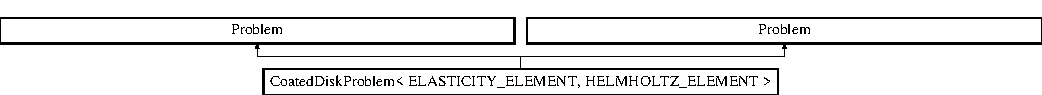
\includegraphics[height=1.272727cm]{classCoatedDiskProblem}
\end{center}
\end{figure}
\subsection*{Public Member Functions}
\begin{DoxyCompactItemize}
\item 
\hyperlink{classCoatedDiskProblem_a9585ca5b422c72dc2b91cbb3e311b736}{Coated\+Disk\+Problem} ()
\begin{DoxyCompactList}\small\item\em Constructor\+: \end{DoxyCompactList}\item 
void \hyperlink{classCoatedDiskProblem_a3b94aaddee6a8f386ba249f418813963}{actions\+\_\+before\+\_\+newton\+\_\+solve} ()
\begin{DoxyCompactList}\small\item\em Update function (empty) \end{DoxyCompactList}\item 
void \hyperlink{classCoatedDiskProblem_aa0b9b4e706cdb1b31738c3db8759e9ee}{actions\+\_\+after\+\_\+newton\+\_\+solve} ()
\begin{DoxyCompactList}\small\item\em Update function (empty) \end{DoxyCompactList}\item 
void \hyperlink{classCoatedDiskProblem_a8f52f13933fba3b053d50de544d8cafc}{actions\+\_\+before\+\_\+newton\+\_\+convergence\+\_\+check} ()
\begin{DoxyCompactList}\small\item\em Recompute gamma integral before checking Newton residuals. \end{DoxyCompactList}\item 
void \hyperlink{classCoatedDiskProblem_a89e972df172b024b1358f0fac7646d6d}{actions\+\_\+before\+\_\+adapt} ()
\begin{DoxyCompactList}\small\item\em Actions before adapt\+: Wipe the mesh of traction elements. \end{DoxyCompactList}\item 
void \hyperlink{classCoatedDiskProblem_a93f9d34cd24f08ca1ec726ae0057b939}{actions\+\_\+after\+\_\+adapt} ()
\begin{DoxyCompactList}\small\item\em Actions after adapt\+: Rebuild the mesh of traction elements. \end{DoxyCompactList}\item 
void \hyperlink{classCoatedDiskProblem_af8e103d494f526c0e24c0c4ccef4ea6b}{doc\+\_\+solution} ()
\begin{DoxyCompactList}\small\item\em Doc the solution. \end{DoxyCompactList}\item 
\hyperlink{classCoatedDiskProblem_a9585ca5b422c72dc2b91cbb3e311b736}{Coated\+Disk\+Problem} ()
\begin{DoxyCompactList}\small\item\em Constructor\+: \end{DoxyCompactList}\item 
void \hyperlink{classCoatedDiskProblem_a3b94aaddee6a8f386ba249f418813963}{actions\+\_\+before\+\_\+newton\+\_\+solve} ()
\begin{DoxyCompactList}\small\item\em Update function (empty) \end{DoxyCompactList}\item 
void \hyperlink{classCoatedDiskProblem_aa0b9b4e706cdb1b31738c3db8759e9ee}{actions\+\_\+after\+\_\+newton\+\_\+solve} ()
\begin{DoxyCompactList}\small\item\em Update function (empty) \end{DoxyCompactList}\item 
void \hyperlink{classCoatedDiskProblem_a89e972df172b024b1358f0fac7646d6d}{actions\+\_\+before\+\_\+adapt} ()
\begin{DoxyCompactList}\small\item\em Actions before adapt\+: Wipe the face meshes. \end{DoxyCompactList}\item 
void \hyperlink{classCoatedDiskProblem_a93f9d34cd24f08ca1ec726ae0057b939}{actions\+\_\+after\+\_\+adapt} ()
\begin{DoxyCompactList}\small\item\em Actions after adapt\+: Rebuild the face meshes. \end{DoxyCompactList}\item 
void \hyperlink{classCoatedDiskProblem_af8e103d494f526c0e24c0c4ccef4ea6b}{doc\+\_\+solution} ()
\begin{DoxyCompactList}\small\item\em Doc the solution. \end{DoxyCompactList}\end{DoxyCompactItemize}
\subsection*{Private Member Functions}
\begin{DoxyCompactItemize}
\item 
void \hyperlink{classCoatedDiskProblem_a143908e8db74ad6bd8b7efaaa26c78c3}{create\+\_\+fsi\+\_\+traction\+\_\+elements} ()
\begin{DoxyCompactList}\small\item\em Create F\+SI traction elements. \end{DoxyCompactList}\item 
void \hyperlink{classCoatedDiskProblem_a34f61c03b152f2ac06e1e771b0dbe09b}{create\+\_\+helmholtz\+\_\+fsi\+\_\+flux\+\_\+elements} ()
\begin{DoxyCompactList}\small\item\em Create Helmholtz F\+SI flux elements. \end{DoxyCompactList}\item 
void \hyperlink{classCoatedDiskProblem_a55b4cead41e01ab5fd728b607f62bb74}{delete\+\_\+face\+\_\+elements} (Mesh $\ast$const \&boundary\+\_\+mesh\+\_\+pt)
\begin{DoxyCompactList}\small\item\em Delete (face) elements in specified mesh. \end{DoxyCompactList}\item 
void \hyperlink{classCoatedDiskProblem_a222b74395afde602617965f60c885491}{create\+\_\+helmholtz\+\_\+\+Dt\+N\+\_\+elements} ()
\begin{DoxyCompactList}\small\item\em Create DtN face elements. \end{DoxyCompactList}\item 
void \hyperlink{classCoatedDiskProblem_ad24d43389155a6a9f2f66faf4b239c26}{setup\+\_\+interaction} ()
\begin{DoxyCompactList}\small\item\em Setup interaction. \end{DoxyCompactList}\item 
void \hyperlink{classCoatedDiskProblem_a4d63252d3916bda71f28b637d6590627}{complete\+\_\+problem\+\_\+setup} ()
\item 
void \hyperlink{classCoatedDiskProblem_a31c3707de78a720e3936e3b34e70b1ba}{create\+\_\+solid\+\_\+traction\+\_\+elements} ()
\begin{DoxyCompactList}\small\item\em Create solid traction elements. \end{DoxyCompactList}\item 
void \hyperlink{classCoatedDiskProblem_a143908e8db74ad6bd8b7efaaa26c78c3}{create\+\_\+fsi\+\_\+traction\+\_\+elements} ()
\begin{DoxyCompactList}\small\item\em Create F\+SI traction elements. \end{DoxyCompactList}\item 
void \hyperlink{classCoatedDiskProblem_a34f61c03b152f2ac06e1e771b0dbe09b}{create\+\_\+helmholtz\+\_\+fsi\+\_\+flux\+\_\+elements} ()
\begin{DoxyCompactList}\small\item\em Create Helmholtz F\+SI flux elements. \end{DoxyCompactList}\item 
void \hyperlink{classCoatedDiskProblem_a55b4cead41e01ab5fd728b607f62bb74}{delete\+\_\+face\+\_\+elements} (Mesh $\ast$const \&boundary\+\_\+mesh\+\_\+pt)
\begin{DoxyCompactList}\small\item\em Delete (face) elements in specified mesh. \end{DoxyCompactList}\item 
void \hyperlink{classCoatedDiskProblem_ade4e1e8fd2e8b0f7592f26514f3d18cc}{create\+\_\+helmholtz\+\_\+\+A\+B\+C\+\_\+elements} ()
\begin{DoxyCompactList}\small\item\em Create A\+BC face elements. \end{DoxyCompactList}\item 
void \hyperlink{classCoatedDiskProblem_ad24d43389155a6a9f2f66faf4b239c26}{setup\+\_\+interaction} ()
\begin{DoxyCompactList}\small\item\em Setup interaction. \end{DoxyCompactList}\end{DoxyCompactItemize}
\subsection*{Private Attributes}
\begin{DoxyCompactItemize}
\item 
Tree\+Based\+Refineable\+Mesh\+Base $\ast$ \hyperlink{classCoatedDiskProblem_aa9e9529dcb4bfd7793b868ab42a5d10e}{Solid\+\_\+mesh\+\_\+pt}
\begin{DoxyCompactList}\small\item\em Pointer to solid mesh. \end{DoxyCompactList}\item 
Mesh $\ast$ \hyperlink{classCoatedDiskProblem_aefeabd04f0fd48be258e57a8b73038b4}{F\+S\+I\+\_\+traction\+\_\+mesh\+\_\+pt}
\begin{DoxyCompactList}\small\item\em Pointer to mesh of F\+SI traction elements. \end{DoxyCompactList}\item 
Tree\+Based\+Refineable\+Mesh\+Base $\ast$ \hyperlink{classCoatedDiskProblem_ad434a37897336e7dfdb720c0b8941c8a}{Helmholtz\+\_\+mesh\+\_\+pt}
\begin{DoxyCompactList}\small\item\em Pointer to Helmholtz mesh. \end{DoxyCompactList}\item 
Mesh $\ast$ \hyperlink{classCoatedDiskProblem_a1737537bbd37b74915e3bfe43e3e4d3e}{Helmholtz\+\_\+fsi\+\_\+flux\+\_\+mesh\+\_\+pt}
\begin{DoxyCompactList}\small\item\em Pointer to mesh of Helmholtz F\+SI flux elements. \end{DoxyCompactList}\item 
Helmholtz\+Dt\+N\+Mesh$<$ H\+E\+L\+M\+H\+O\+L\+T\+Z\+\_\+\+E\+L\+E\+M\+E\+NT $>$ $\ast$ \hyperlink{classCoatedDiskProblem_a142852ffdecdb2f76acf3e4c11ce4b04}{Helmholtz\+\_\+outer\+\_\+boundary\+\_\+mesh\+\_\+pt}
\begin{DoxyCompactList}\small\item\em Pointer to mesh containing the DtN elements. \end{DoxyCompactList}\item 
Doc\+Info \hyperlink{classCoatedDiskProblem_ab389fe08ad443c10ddbdd12127903477}{Doc\+\_\+info}
\begin{DoxyCompactList}\small\item\em Doc\+Info object for output. \end{DoxyCompactList}\item 
ofstream \hyperlink{classCoatedDiskProblem_a5a6336e64a200817fedd99a333d2c0be}{Trace\+\_\+file}
\begin{DoxyCompactList}\small\item\em Trace file. \end{DoxyCompactList}\item 
Refineable\+Triangle\+Mesh$<$ E\+L\+A\+S\+T\+I\+C\+I\+T\+Y\+\_\+\+E\+L\+E\+M\+E\+NT $>$ $\ast$ \hyperlink{classCoatedDiskProblem_a9121e4e334b9570dd19c5b011b726eb7}{Solid\+\_\+mesh\+\_\+pt}
\begin{DoxyCompactList}\small\item\em Pointer to refineable solid mesh. \end{DoxyCompactList}\item 
Mesh $\ast$ \hyperlink{classCoatedDiskProblem_a40be95c16554cc776ee45129c9153cae}{Solid\+\_\+traction\+\_\+mesh\+\_\+pt}
\begin{DoxyCompactList}\small\item\em Pointer to mesh of solid traction elements. \end{DoxyCompactList}\item 
Mesh $\ast$ \hyperlink{classCoatedDiskProblem_a2e3b9aaa75f8ce03625aeaf7a4ea7c77}{Helmholtz\+\_\+outer\+\_\+boundary\+\_\+mesh\+\_\+pt}
\begin{DoxyCompactList}\small\item\em Pointer to mesh containing the A\+BC elements. \end{DoxyCompactList}\item 
unsigned \hyperlink{classCoatedDiskProblem_ab0fb6d4bdf876fb2df1f2fa05606526b}{Upper\+\_\+symmetry\+\_\+boundary\+\_\+id}
\begin{DoxyCompactList}\small\item\em Boundary ID of upper symmetry boundary. \end{DoxyCompactList}\item 
unsigned \hyperlink{classCoatedDiskProblem_a42d2f2b46b0b1a7add92533bd5968033}{Lower\+\_\+symmetry\+\_\+boundary\+\_\+id}
\begin{DoxyCompactList}\small\item\em Boundary ID of lower symmetry boundary. \end{DoxyCompactList}\item 
unsigned \hyperlink{classCoatedDiskProblem_ae22c200ea010aa2420b96c2592034cd5}{Upper\+\_\+inner\+\_\+boundary\+\_\+id}
\begin{DoxyCompactList}\small\item\em Boundary ID of upper inner boundary. \end{DoxyCompactList}\item 
unsigned \hyperlink{classCoatedDiskProblem_a693be7a3e4c968c52d5c19d9a35a05b3}{Lower\+\_\+inner\+\_\+boundary\+\_\+id}
\begin{DoxyCompactList}\small\item\em Boundary ID of lower inner boundary. \end{DoxyCompactList}\item 
unsigned \hyperlink{classCoatedDiskProblem_acdffaaa300e0c67b5ceb7c85925a46f0}{Outer\+\_\+boundary\+\_\+id}
\begin{DoxyCompactList}\small\item\em Boundary ID of outer boundary. \end{DoxyCompactList}\item 
unsigned \hyperlink{classCoatedDiskProblem_a0f241ef5043d002c90d68a93831e9212}{Rib\+\_\+divider\+\_\+boundary\+\_\+id}
\end{DoxyCompactItemize}


\subsection{Detailed Description}
\subsubsection*{template$<$class E\+L\+A\+S\+T\+I\+C\+I\+T\+Y\+\_\+\+E\+L\+E\+M\+E\+NT, class H\+E\+L\+M\+H\+O\+L\+T\+Z\+\_\+\+E\+L\+E\+M\+E\+NT$>$\newline
class Coated\+Disk\+Problem$<$ E\+L\+A\+S\+T\+I\+C\+I\+T\+Y\+\_\+\+E\+L\+E\+M\+E\+N\+T, H\+E\+L\+M\+H\+O\+L\+T\+Z\+\_\+\+E\+L\+E\+M\+E\+N\+T $>$}

Coated disk F\+SI. 

Definition at line 239 of file acoustic\+\_\+fsi.\+cc.



\subsection{Constructor \& Destructor Documentation}
\mbox{\Hypertarget{classCoatedDiskProblem_a9585ca5b422c72dc2b91cbb3e311b736}\label{classCoatedDiskProblem_a9585ca5b422c72dc2b91cbb3e311b736}} 
\index{Coated\+Disk\+Problem@{Coated\+Disk\+Problem}!Coated\+Disk\+Problem@{Coated\+Disk\+Problem}}
\index{Coated\+Disk\+Problem@{Coated\+Disk\+Problem}!Coated\+Disk\+Problem@{Coated\+Disk\+Problem}}
\subsubsection{\texorpdfstring{Coated\+Disk\+Problem()}{CoatedDiskProblem()}\hspace{0.1cm}{\footnotesize\ttfamily [1/2]}}
{\footnotesize\ttfamily template$<$class E\+L\+A\+S\+T\+I\+C\+I\+T\+Y\+\_\+\+E\+L\+E\+M\+E\+NT , class H\+E\+L\+M\+H\+O\+L\+T\+Z\+\_\+\+E\+L\+E\+M\+E\+NT $>$ \\
\hyperlink{classCoatedDiskProblem}{Coated\+Disk\+Problem}$<$ E\+L\+A\+S\+T\+I\+C\+I\+T\+Y\+\_\+\+E\+L\+E\+M\+E\+NT, H\+E\+L\+M\+H\+O\+L\+T\+Z\+\_\+\+E\+L\+E\+M\+E\+NT $>$\+::\hyperlink{classCoatedDiskProblem}{Coated\+Disk\+Problem} (\begin{DoxyParamCaption}{ }\end{DoxyParamCaption})}



Constructor\+: 

Constructor. 

Definition at line 313 of file acoustic\+\_\+fsi.\+cc.



References Coated\+Disk\+Problem$<$ E\+L\+A\+S\+T\+I\+C\+I\+T\+Y\+\_\+\+E\+L\+E\+M\+E\+N\+T, H\+E\+L\+M\+H\+O\+L\+T\+Z\+\_\+\+E\+L\+E\+M\+E\+N\+T $>$\+::actions\+\_\+before\+\_\+adapt(), Global\+\_\+\+Parameters\+::\+Directory, Global\+\_\+\+Parameters\+::\+E(), Global\+\_\+\+Parameters\+::\+El\+\_\+multiplier, Global\+\_\+\+Parameters\+::\+H\+\_\+coating, Global\+\_\+\+Parameters\+::\+K\+\_\+squared, Global\+\_\+\+Parameters\+::\+Omega\+\_\+sq, Global\+\_\+\+Parameters\+::\+Outer\+\_\+radius, and Global\+\_\+\+Parameters\+::solid\+\_\+boundary\+\_\+displacement().

\mbox{\Hypertarget{classCoatedDiskProblem_a9585ca5b422c72dc2b91cbb3e311b736}\label{classCoatedDiskProblem_a9585ca5b422c72dc2b91cbb3e311b736}} 
\index{Coated\+Disk\+Problem@{Coated\+Disk\+Problem}!Coated\+Disk\+Problem@{Coated\+Disk\+Problem}}
\index{Coated\+Disk\+Problem@{Coated\+Disk\+Problem}!Coated\+Disk\+Problem@{Coated\+Disk\+Problem}}
\subsubsection{\texorpdfstring{Coated\+Disk\+Problem()}{CoatedDiskProblem()}\hspace{0.1cm}{\footnotesize\ttfamily [2/2]}}
{\footnotesize\ttfamily template$<$class E\+L\+A\+S\+T\+I\+C\+I\+T\+Y\+\_\+\+E\+L\+E\+M\+E\+NT, class H\+E\+L\+M\+H\+O\+L\+T\+Z\+\_\+\+E\+L\+E\+M\+E\+NT$>$ \\
\hyperlink{classCoatedDiskProblem}{Coated\+Disk\+Problem}$<$ E\+L\+A\+S\+T\+I\+C\+I\+T\+Y\+\_\+\+E\+L\+E\+M\+E\+NT, H\+E\+L\+M\+H\+O\+L\+T\+Z\+\_\+\+E\+L\+E\+M\+E\+NT $>$\+::\hyperlink{classCoatedDiskProblem}{Coated\+Disk\+Problem} (\begin{DoxyParamCaption}{ }\end{DoxyParamCaption})}



Constructor\+: 



\subsection{Member Function Documentation}
\mbox{\Hypertarget{classCoatedDiskProblem_a93f9d34cd24f08ca1ec726ae0057b939}\label{classCoatedDiskProblem_a93f9d34cd24f08ca1ec726ae0057b939}} 
\index{Coated\+Disk\+Problem@{Coated\+Disk\+Problem}!actions\+\_\+after\+\_\+adapt@{actions\+\_\+after\+\_\+adapt}}
\index{actions\+\_\+after\+\_\+adapt@{actions\+\_\+after\+\_\+adapt}!Coated\+Disk\+Problem@{Coated\+Disk\+Problem}}
\subsubsection{\texorpdfstring{actions\+\_\+after\+\_\+adapt()}{actions\_after\_adapt()}\hspace{0.1cm}{\footnotesize\ttfamily [1/2]}}
{\footnotesize\ttfamily template$<$class E\+L\+A\+S\+T\+I\+C\+I\+T\+Y\+\_\+\+E\+L\+E\+M\+E\+NT, class H\+E\+L\+M\+H\+O\+L\+T\+Z\+\_\+\+E\+L\+E\+M\+E\+NT$>$ \\
void \hyperlink{classCoatedDiskProblem}{Coated\+Disk\+Problem}$<$ E\+L\+A\+S\+T\+I\+C\+I\+T\+Y\+\_\+\+E\+L\+E\+M\+E\+NT, H\+E\+L\+M\+H\+O\+L\+T\+Z\+\_\+\+E\+L\+E\+M\+E\+NT $>$\+::actions\+\_\+after\+\_\+adapt (\begin{DoxyParamCaption}{ }\end{DoxyParamCaption})}



Actions after adapt\+: Rebuild the face meshes. 

\mbox{\Hypertarget{classCoatedDiskProblem_a93f9d34cd24f08ca1ec726ae0057b939}\label{classCoatedDiskProblem_a93f9d34cd24f08ca1ec726ae0057b939}} 
\index{Coated\+Disk\+Problem@{Coated\+Disk\+Problem}!actions\+\_\+after\+\_\+adapt@{actions\+\_\+after\+\_\+adapt}}
\index{actions\+\_\+after\+\_\+adapt@{actions\+\_\+after\+\_\+adapt}!Coated\+Disk\+Problem@{Coated\+Disk\+Problem}}
\subsubsection{\texorpdfstring{actions\+\_\+after\+\_\+adapt()}{actions\_after\_adapt()}\hspace{0.1cm}{\footnotesize\ttfamily [2/2]}}
{\footnotesize\ttfamily template$<$class E\+L\+A\+S\+T\+I\+C\+I\+T\+Y\+\_\+\+E\+L\+E\+M\+E\+NT , class H\+E\+L\+M\+H\+O\+L\+T\+Z\+\_\+\+E\+L\+E\+M\+E\+NT $>$ \\
void \hyperlink{classCoatedDiskProblem}{Coated\+Disk\+Problem}$<$ E\+L\+A\+S\+T\+I\+C\+I\+T\+Y\+\_\+\+E\+L\+E\+M\+E\+NT, H\+E\+L\+M\+H\+O\+L\+T\+Z\+\_\+\+E\+L\+E\+M\+E\+NT $>$\+::actions\+\_\+after\+\_\+adapt (\begin{DoxyParamCaption}{ }\end{DoxyParamCaption})}



Actions after adapt\+: Rebuild the mesh of traction elements. 

Actions after adapt\+: Rebuild the meshes of face elements. 

Definition at line 528 of file acoustic\+\_\+fsi.\+cc.



References Coated\+Disk\+Problem$<$ E\+L\+A\+S\+T\+I\+C\+I\+T\+Y\+\_\+\+E\+L\+E\+M\+E\+N\+T, H\+E\+L\+M\+H\+O\+L\+T\+Z\+\_\+\+E\+L\+E\+M\+E\+N\+T $>$\+::delete\+\_\+face\+\_\+elements().



Referenced by Coated\+Disk\+Problem$<$ E\+L\+A\+S\+T\+I\+C\+I\+T\+Y\+\_\+\+E\+L\+E\+M\+E\+N\+T, H\+E\+L\+M\+H\+O\+L\+T\+Z\+\_\+\+E\+L\+E\+M\+E\+N\+T $>$\+::actions\+\_\+before\+\_\+adapt().

\mbox{\Hypertarget{classCoatedDiskProblem_aa0b9b4e706cdb1b31738c3db8759e9ee}\label{classCoatedDiskProblem_aa0b9b4e706cdb1b31738c3db8759e9ee}} 
\index{Coated\+Disk\+Problem@{Coated\+Disk\+Problem}!actions\+\_\+after\+\_\+newton\+\_\+solve@{actions\+\_\+after\+\_\+newton\+\_\+solve}}
\index{actions\+\_\+after\+\_\+newton\+\_\+solve@{actions\+\_\+after\+\_\+newton\+\_\+solve}!Coated\+Disk\+Problem@{Coated\+Disk\+Problem}}
\subsubsection{\texorpdfstring{actions\+\_\+after\+\_\+newton\+\_\+solve()}{actions\_after\_newton\_solve()}\hspace{0.1cm}{\footnotesize\ttfamily [1/2]}}
{\footnotesize\ttfamily template$<$class E\+L\+A\+S\+T\+I\+C\+I\+T\+Y\+\_\+\+E\+L\+E\+M\+E\+NT, class H\+E\+L\+M\+H\+O\+L\+T\+Z\+\_\+\+E\+L\+E\+M\+E\+NT$>$ \\
void \hyperlink{classCoatedDiskProblem}{Coated\+Disk\+Problem}$<$ E\+L\+A\+S\+T\+I\+C\+I\+T\+Y\+\_\+\+E\+L\+E\+M\+E\+NT, H\+E\+L\+M\+H\+O\+L\+T\+Z\+\_\+\+E\+L\+E\+M\+E\+NT $>$\+::actions\+\_\+after\+\_\+newton\+\_\+solve (\begin{DoxyParamCaption}{ }\end{DoxyParamCaption})\hspace{0.3cm}{\ttfamily [inline]}}



Update function (empty) 



Definition at line 195 of file unstructured\+\_\+acoustic\+\_\+fsi.\+cc.

\mbox{\Hypertarget{classCoatedDiskProblem_aa0b9b4e706cdb1b31738c3db8759e9ee}\label{classCoatedDiskProblem_aa0b9b4e706cdb1b31738c3db8759e9ee}} 
\index{Coated\+Disk\+Problem@{Coated\+Disk\+Problem}!actions\+\_\+after\+\_\+newton\+\_\+solve@{actions\+\_\+after\+\_\+newton\+\_\+solve}}
\index{actions\+\_\+after\+\_\+newton\+\_\+solve@{actions\+\_\+after\+\_\+newton\+\_\+solve}!Coated\+Disk\+Problem@{Coated\+Disk\+Problem}}
\subsubsection{\texorpdfstring{actions\+\_\+after\+\_\+newton\+\_\+solve()}{actions\_after\_newton\_solve()}\hspace{0.1cm}{\footnotesize\ttfamily [2/2]}}
{\footnotesize\ttfamily template$<$class E\+L\+A\+S\+T\+I\+C\+I\+T\+Y\+\_\+\+E\+L\+E\+M\+E\+NT, class H\+E\+L\+M\+H\+O\+L\+T\+Z\+\_\+\+E\+L\+E\+M\+E\+NT$>$ \\
void \hyperlink{classCoatedDiskProblem}{Coated\+Disk\+Problem}$<$ E\+L\+A\+S\+T\+I\+C\+I\+T\+Y\+\_\+\+E\+L\+E\+M\+E\+NT, H\+E\+L\+M\+H\+O\+L\+T\+Z\+\_\+\+E\+L\+E\+M\+E\+NT $>$\+::actions\+\_\+after\+\_\+newton\+\_\+solve (\begin{DoxyParamCaption}{ }\end{DoxyParamCaption})\hspace{0.3cm}{\ttfamily [inline]}}



Update function (empty) 



Definition at line 251 of file acoustic\+\_\+fsi.\+cc.

\mbox{\Hypertarget{classCoatedDiskProblem_a89e972df172b024b1358f0fac7646d6d}\label{classCoatedDiskProblem_a89e972df172b024b1358f0fac7646d6d}} 
\index{Coated\+Disk\+Problem@{Coated\+Disk\+Problem}!actions\+\_\+before\+\_\+adapt@{actions\+\_\+before\+\_\+adapt}}
\index{actions\+\_\+before\+\_\+adapt@{actions\+\_\+before\+\_\+adapt}!Coated\+Disk\+Problem@{Coated\+Disk\+Problem}}
\subsubsection{\texorpdfstring{actions\+\_\+before\+\_\+adapt()}{actions\_before\_adapt()}\hspace{0.1cm}{\footnotesize\ttfamily [1/2]}}
{\footnotesize\ttfamily template$<$class E\+L\+A\+S\+T\+I\+C\+I\+T\+Y\+\_\+\+E\+L\+E\+M\+E\+NT, class H\+E\+L\+M\+H\+O\+L\+T\+Z\+\_\+\+E\+L\+E\+M\+E\+NT$>$ \\
void \hyperlink{classCoatedDiskProblem}{Coated\+Disk\+Problem}$<$ E\+L\+A\+S\+T\+I\+C\+I\+T\+Y\+\_\+\+E\+L\+E\+M\+E\+NT, H\+E\+L\+M\+H\+O\+L\+T\+Z\+\_\+\+E\+L\+E\+M\+E\+NT $>$\+::actions\+\_\+before\+\_\+adapt (\begin{DoxyParamCaption}{ }\end{DoxyParamCaption})}



Actions before adapt\+: Wipe the face meshes. 

\mbox{\Hypertarget{classCoatedDiskProblem_a89e972df172b024b1358f0fac7646d6d}\label{classCoatedDiskProblem_a89e972df172b024b1358f0fac7646d6d}} 
\index{Coated\+Disk\+Problem@{Coated\+Disk\+Problem}!actions\+\_\+before\+\_\+adapt@{actions\+\_\+before\+\_\+adapt}}
\index{actions\+\_\+before\+\_\+adapt@{actions\+\_\+before\+\_\+adapt}!Coated\+Disk\+Problem@{Coated\+Disk\+Problem}}
\subsubsection{\texorpdfstring{actions\+\_\+before\+\_\+adapt()}{actions\_before\_adapt()}\hspace{0.1cm}{\footnotesize\ttfamily [2/2]}}
{\footnotesize\ttfamily template$<$class E\+L\+A\+S\+T\+I\+C\+I\+T\+Y\+\_\+\+E\+L\+E\+M\+E\+NT , class H\+E\+L\+M\+H\+O\+L\+T\+Z\+\_\+\+E\+L\+E\+M\+E\+NT $>$ \\
void \hyperlink{classCoatedDiskProblem}{Coated\+Disk\+Problem}$<$ E\+L\+A\+S\+T\+I\+C\+I\+T\+Y\+\_\+\+E\+L\+E\+M\+E\+NT, H\+E\+L\+M\+H\+O\+L\+T\+Z\+\_\+\+E\+L\+E\+M\+E\+NT $>$\+::actions\+\_\+before\+\_\+adapt (\begin{DoxyParamCaption}{ }\end{DoxyParamCaption})}



Actions before adapt\+: Wipe the mesh of traction elements. 

Actions before adapt\+: Wipe the meshes face elements. 

Definition at line 505 of file acoustic\+\_\+fsi.\+cc.



References Coated\+Disk\+Problem$<$ E\+L\+A\+S\+T\+I\+C\+I\+T\+Y\+\_\+\+E\+L\+E\+M\+E\+N\+T, H\+E\+L\+M\+H\+O\+L\+T\+Z\+\_\+\+E\+L\+E\+M\+E\+N\+T $>$\+::actions\+\_\+after\+\_\+adapt().



Referenced by Coated\+Disk\+Problem$<$ E\+L\+A\+S\+T\+I\+C\+I\+T\+Y\+\_\+\+E\+L\+E\+M\+E\+N\+T, H\+E\+L\+M\+H\+O\+L\+T\+Z\+\_\+\+E\+L\+E\+M\+E\+N\+T $>$\+::\+Coated\+Disk\+Problem().

\mbox{\Hypertarget{classCoatedDiskProblem_a8f52f13933fba3b053d50de544d8cafc}\label{classCoatedDiskProblem_a8f52f13933fba3b053d50de544d8cafc}} 
\index{Coated\+Disk\+Problem@{Coated\+Disk\+Problem}!actions\+\_\+before\+\_\+newton\+\_\+convergence\+\_\+check@{actions\+\_\+before\+\_\+newton\+\_\+convergence\+\_\+check}}
\index{actions\+\_\+before\+\_\+newton\+\_\+convergence\+\_\+check@{actions\+\_\+before\+\_\+newton\+\_\+convergence\+\_\+check}!Coated\+Disk\+Problem@{Coated\+Disk\+Problem}}
\subsubsection{\texorpdfstring{actions\+\_\+before\+\_\+newton\+\_\+convergence\+\_\+check()}{actions\_before\_newton\_convergence\_check()}}
{\footnotesize\ttfamily template$<$class E\+L\+A\+S\+T\+I\+C\+I\+T\+Y\+\_\+\+E\+L\+E\+M\+E\+NT, class H\+E\+L\+M\+H\+O\+L\+T\+Z\+\_\+\+E\+L\+E\+M\+E\+NT$>$ \\
void \hyperlink{classCoatedDiskProblem}{Coated\+Disk\+Problem}$<$ E\+L\+A\+S\+T\+I\+C\+I\+T\+Y\+\_\+\+E\+L\+E\+M\+E\+NT, H\+E\+L\+M\+H\+O\+L\+T\+Z\+\_\+\+E\+L\+E\+M\+E\+NT $>$\+::actions\+\_\+before\+\_\+newton\+\_\+convergence\+\_\+check (\begin{DoxyParamCaption}{ }\end{DoxyParamCaption})\hspace{0.3cm}{\ttfamily [inline]}}



Recompute gamma integral before checking Newton residuals. 



Definition at line 254 of file acoustic\+\_\+fsi.\+cc.

\mbox{\Hypertarget{classCoatedDiskProblem_a3b94aaddee6a8f386ba249f418813963}\label{classCoatedDiskProblem_a3b94aaddee6a8f386ba249f418813963}} 
\index{Coated\+Disk\+Problem@{Coated\+Disk\+Problem}!actions\+\_\+before\+\_\+newton\+\_\+solve@{actions\+\_\+before\+\_\+newton\+\_\+solve}}
\index{actions\+\_\+before\+\_\+newton\+\_\+solve@{actions\+\_\+before\+\_\+newton\+\_\+solve}!Coated\+Disk\+Problem@{Coated\+Disk\+Problem}}
\subsubsection{\texorpdfstring{actions\+\_\+before\+\_\+newton\+\_\+solve()}{actions\_before\_newton\_solve()}\hspace{0.1cm}{\footnotesize\ttfamily [1/2]}}
{\footnotesize\ttfamily template$<$class E\+L\+A\+S\+T\+I\+C\+I\+T\+Y\+\_\+\+E\+L\+E\+M\+E\+NT, class H\+E\+L\+M\+H\+O\+L\+T\+Z\+\_\+\+E\+L\+E\+M\+E\+NT$>$ \\
void \hyperlink{classCoatedDiskProblem}{Coated\+Disk\+Problem}$<$ E\+L\+A\+S\+T\+I\+C\+I\+T\+Y\+\_\+\+E\+L\+E\+M\+E\+NT, H\+E\+L\+M\+H\+O\+L\+T\+Z\+\_\+\+E\+L\+E\+M\+E\+NT $>$\+::actions\+\_\+before\+\_\+newton\+\_\+solve (\begin{DoxyParamCaption}{ }\end{DoxyParamCaption})\hspace{0.3cm}{\ttfamily [inline]}}



Update function (empty) 



Definition at line 192 of file unstructured\+\_\+acoustic\+\_\+fsi.\+cc.

\mbox{\Hypertarget{classCoatedDiskProblem_a3b94aaddee6a8f386ba249f418813963}\label{classCoatedDiskProblem_a3b94aaddee6a8f386ba249f418813963}} 
\index{Coated\+Disk\+Problem@{Coated\+Disk\+Problem}!actions\+\_\+before\+\_\+newton\+\_\+solve@{actions\+\_\+before\+\_\+newton\+\_\+solve}}
\index{actions\+\_\+before\+\_\+newton\+\_\+solve@{actions\+\_\+before\+\_\+newton\+\_\+solve}!Coated\+Disk\+Problem@{Coated\+Disk\+Problem}}
\subsubsection{\texorpdfstring{actions\+\_\+before\+\_\+newton\+\_\+solve()}{actions\_before\_newton\_solve()}\hspace{0.1cm}{\footnotesize\ttfamily [2/2]}}
{\footnotesize\ttfamily template$<$class E\+L\+A\+S\+T\+I\+C\+I\+T\+Y\+\_\+\+E\+L\+E\+M\+E\+NT, class H\+E\+L\+M\+H\+O\+L\+T\+Z\+\_\+\+E\+L\+E\+M\+E\+NT$>$ \\
void \hyperlink{classCoatedDiskProblem}{Coated\+Disk\+Problem}$<$ E\+L\+A\+S\+T\+I\+C\+I\+T\+Y\+\_\+\+E\+L\+E\+M\+E\+NT, H\+E\+L\+M\+H\+O\+L\+T\+Z\+\_\+\+E\+L\+E\+M\+E\+NT $>$\+::actions\+\_\+before\+\_\+newton\+\_\+solve (\begin{DoxyParamCaption}{ }\end{DoxyParamCaption})\hspace{0.3cm}{\ttfamily [inline]}}



Update function (empty) 



Definition at line 248 of file acoustic\+\_\+fsi.\+cc.

\mbox{\Hypertarget{classCoatedDiskProblem_a4d63252d3916bda71f28b637d6590627}\label{classCoatedDiskProblem_a4d63252d3916bda71f28b637d6590627}} 
\index{Coated\+Disk\+Problem@{Coated\+Disk\+Problem}!complete\+\_\+problem\+\_\+setup@{complete\+\_\+problem\+\_\+setup}}
\index{complete\+\_\+problem\+\_\+setup@{complete\+\_\+problem\+\_\+setup}!Coated\+Disk\+Problem@{Coated\+Disk\+Problem}}
\subsubsection{\texorpdfstring{complete\+\_\+problem\+\_\+setup()}{complete\_problem\_setup()}}
{\footnotesize\ttfamily template$<$class E\+L\+A\+S\+T\+I\+C\+I\+T\+Y\+\_\+\+E\+L\+E\+M\+E\+NT , class H\+E\+L\+M\+H\+O\+L\+T\+Z\+\_\+\+E\+L\+E\+M\+E\+NT $>$ \\
void \hyperlink{classCoatedDiskProblem}{Coated\+Disk\+Problem}$<$ E\+L\+A\+S\+T\+I\+C\+I\+T\+Y\+\_\+\+E\+L\+E\+M\+E\+NT, H\+E\+L\+M\+H\+O\+L\+T\+Z\+\_\+\+E\+L\+E\+M\+E\+NT $>$\+::complete\+\_\+problem\+\_\+setup (\begin{DoxyParamCaption}{ }\end{DoxyParamCaption})\hspace{0.3cm}{\ttfamily [private]}}

Complete problem setup\+: Apply boundary conditions and set physical properties 

Definition at line 774 of file unstructured\+\_\+acoustic\+\_\+fsi.\+cc.



References Coated\+Disk\+Problem$<$ E\+L\+A\+S\+T\+I\+C\+I\+T\+Y\+\_\+\+E\+L\+E\+M\+E\+N\+T, H\+E\+L\+M\+H\+O\+L\+T\+Z\+\_\+\+E\+L\+E\+M\+E\+N\+T $>$\+::create\+\_\+solid\+\_\+traction\+\_\+elements(), Coated\+Disk\+Problem$<$ E\+L\+A\+S\+T\+I\+C\+I\+T\+Y\+\_\+\+E\+L\+E\+M\+E\+N\+T, H\+E\+L\+M\+H\+O\+L\+T\+Z\+\_\+\+E\+L\+E\+M\+E\+N\+T $>$\+::delete\+\_\+face\+\_\+elements(), Global\+\_\+\+Parameters\+::\+E\+\_\+pt, and Global\+\_\+\+Parameters\+::\+Omega\+\_\+sq.

\mbox{\Hypertarget{classCoatedDiskProblem_a143908e8db74ad6bd8b7efaaa26c78c3}\label{classCoatedDiskProblem_a143908e8db74ad6bd8b7efaaa26c78c3}} 
\index{Coated\+Disk\+Problem@{Coated\+Disk\+Problem}!create\+\_\+fsi\+\_\+traction\+\_\+elements@{create\+\_\+fsi\+\_\+traction\+\_\+elements}}
\index{create\+\_\+fsi\+\_\+traction\+\_\+elements@{create\+\_\+fsi\+\_\+traction\+\_\+elements}!Coated\+Disk\+Problem@{Coated\+Disk\+Problem}}
\subsubsection{\texorpdfstring{create\+\_\+fsi\+\_\+traction\+\_\+elements()}{create\_fsi\_traction\_elements()}\hspace{0.1cm}{\footnotesize\ttfamily [1/2]}}
{\footnotesize\ttfamily template$<$class E\+L\+A\+S\+T\+I\+C\+I\+T\+Y\+\_\+\+E\+L\+E\+M\+E\+NT, class H\+E\+L\+M\+H\+O\+L\+T\+Z\+\_\+\+E\+L\+E\+M\+E\+NT$>$ \\
void \hyperlink{classCoatedDiskProblem}{Coated\+Disk\+Problem}$<$ E\+L\+A\+S\+T\+I\+C\+I\+T\+Y\+\_\+\+E\+L\+E\+M\+E\+NT, H\+E\+L\+M\+H\+O\+L\+T\+Z\+\_\+\+E\+L\+E\+M\+E\+NT $>$\+::create\+\_\+fsi\+\_\+traction\+\_\+elements (\begin{DoxyParamCaption}{ }\end{DoxyParamCaption})\hspace{0.3cm}{\ttfamily [private]}}



Create F\+SI traction elements. 

\mbox{\Hypertarget{classCoatedDiskProblem_a143908e8db74ad6bd8b7efaaa26c78c3}\label{classCoatedDiskProblem_a143908e8db74ad6bd8b7efaaa26c78c3}} 
\index{Coated\+Disk\+Problem@{Coated\+Disk\+Problem}!create\+\_\+fsi\+\_\+traction\+\_\+elements@{create\+\_\+fsi\+\_\+traction\+\_\+elements}}
\index{create\+\_\+fsi\+\_\+traction\+\_\+elements@{create\+\_\+fsi\+\_\+traction\+\_\+elements}!Coated\+Disk\+Problem@{Coated\+Disk\+Problem}}
\subsubsection{\texorpdfstring{create\+\_\+fsi\+\_\+traction\+\_\+elements()}{create\_fsi\_traction\_elements()}\hspace{0.1cm}{\footnotesize\ttfamily [2/2]}}
{\footnotesize\ttfamily template$<$class E\+L\+A\+S\+T\+I\+C\+I\+T\+Y\+\_\+\+E\+L\+E\+M\+E\+NT , class H\+E\+L\+M\+H\+O\+L\+T\+Z\+\_\+\+E\+L\+E\+M\+E\+NT $>$ \\
void \hyperlink{classCoatedDiskProblem}{Coated\+Disk\+Problem}$<$ E\+L\+A\+S\+T\+I\+C\+I\+T\+Y\+\_\+\+E\+L\+E\+M\+E\+NT, H\+E\+L\+M\+H\+O\+L\+T\+Z\+\_\+\+E\+L\+E\+M\+E\+NT $>$\+::create\+\_\+fsi\+\_\+traction\+\_\+elements (\begin{DoxyParamCaption}{ }\end{DoxyParamCaption})\hspace{0.3cm}{\ttfamily [private]}}



Create F\+SI traction elements. 

Create fsi traction elements. 

Definition at line 579 of file acoustic\+\_\+fsi.\+cc.



References Coated\+Disk\+Problem$<$ E\+L\+A\+S\+T\+I\+C\+I\+T\+Y\+\_\+\+E\+L\+E\+M\+E\+N\+T, H\+E\+L\+M\+H\+O\+L\+T\+Z\+\_\+\+E\+L\+E\+M\+E\+N\+T $>$\+::create\+\_\+helmholtz\+\_\+fsi\+\_\+flux\+\_\+elements(), and Global\+\_\+\+Parameters\+::Q.



Referenced by Coated\+Disk\+Problem$<$ E\+L\+A\+S\+T\+I\+C\+I\+T\+Y\+\_\+\+E\+L\+E\+M\+E\+N\+T, H\+E\+L\+M\+H\+O\+L\+T\+Z\+\_\+\+E\+L\+E\+M\+E\+N\+T $>$\+::create\+\_\+solid\+\_\+traction\+\_\+elements(), and Coated\+Disk\+Problem$<$ E\+L\+A\+S\+T\+I\+C\+I\+T\+Y\+\_\+\+E\+L\+E\+M\+E\+N\+T, H\+E\+L\+M\+H\+O\+L\+T\+Z\+\_\+\+E\+L\+E\+M\+E\+N\+T $>$\+::delete\+\_\+face\+\_\+elements().

\mbox{\Hypertarget{classCoatedDiskProblem_ade4e1e8fd2e8b0f7592f26514f3d18cc}\label{classCoatedDiskProblem_ade4e1e8fd2e8b0f7592f26514f3d18cc}} 
\index{Coated\+Disk\+Problem@{Coated\+Disk\+Problem}!create\+\_\+helmholtz\+\_\+\+A\+B\+C\+\_\+elements@{create\+\_\+helmholtz\+\_\+\+A\+B\+C\+\_\+elements}}
\index{create\+\_\+helmholtz\+\_\+\+A\+B\+C\+\_\+elements@{create\+\_\+helmholtz\+\_\+\+A\+B\+C\+\_\+elements}!Coated\+Disk\+Problem@{Coated\+Disk\+Problem}}
\subsubsection{\texorpdfstring{create\+\_\+helmholtz\+\_\+\+A\+B\+C\+\_\+elements()}{create\_helmholtz\_ABC\_elements()}}
{\footnotesize\ttfamily template$<$class E\+L\+A\+S\+T\+I\+C\+I\+T\+Y\+\_\+\+E\+L\+E\+M\+E\+NT , class H\+E\+L\+M\+H\+O\+L\+T\+Z\+\_\+\+E\+L\+E\+M\+E\+NT $>$ \\
void \hyperlink{classCoatedDiskProblem}{Coated\+Disk\+Problem}$<$ E\+L\+A\+S\+T\+I\+C\+I\+T\+Y\+\_\+\+E\+L\+E\+M\+E\+NT, H\+E\+L\+M\+H\+O\+L\+T\+Z\+\_\+\+E\+L\+E\+M\+E\+NT $>$\+::create\+\_\+helmholtz\+\_\+\+A\+B\+C\+\_\+elements (\begin{DoxyParamCaption}{ }\end{DoxyParamCaption})\hspace{0.3cm}{\ttfamily [private]}}



Create A\+BC face elements. 

Create A\+BC elements on the outer boundary of the Helmholtz mesh 

Definition at line 1025 of file unstructured\+\_\+acoustic\+\_\+fsi.\+cc.



References Global\+\_\+\+Parameters\+::\+A\+B\+C\+\_\+order, Global\+\_\+\+Parameters\+::\+Density\+\_\+ratio, Coated\+Disk\+Problem$<$ E\+L\+A\+S\+T\+I\+C\+I\+T\+Y\+\_\+\+E\+L\+E\+M\+E\+N\+T, H\+E\+L\+M\+H\+O\+L\+T\+Z\+\_\+\+E\+L\+E\+M\+E\+N\+T $>$\+::doc\+\_\+solution(), Global\+\_\+\+Parameters\+::\+K\+\_\+squared, Global\+\_\+\+Parameters\+::\+Omega\+\_\+sq, Global\+\_\+\+Parameters\+::\+Outer\+\_\+radius, Global\+\_\+\+Parameters\+::Q, and Coated\+Disk\+Problem$<$ E\+L\+A\+S\+T\+I\+C\+I\+T\+Y\+\_\+\+E\+L\+E\+M\+E\+N\+T, H\+E\+L\+M\+H\+O\+L\+T\+Z\+\_\+\+E\+L\+E\+M\+E\+N\+T $>$\+::setup\+\_\+interaction().



Referenced by Coated\+Disk\+Problem$<$ E\+L\+A\+S\+T\+I\+C\+I\+T\+Y\+\_\+\+E\+L\+E\+M\+E\+N\+T, H\+E\+L\+M\+H\+O\+L\+T\+Z\+\_\+\+E\+L\+E\+M\+E\+N\+T $>$\+::create\+\_\+solid\+\_\+traction\+\_\+elements().

\mbox{\Hypertarget{classCoatedDiskProblem_a222b74395afde602617965f60c885491}\label{classCoatedDiskProblem_a222b74395afde602617965f60c885491}} 
\index{Coated\+Disk\+Problem@{Coated\+Disk\+Problem}!create\+\_\+helmholtz\+\_\+\+Dt\+N\+\_\+elements@{create\+\_\+helmholtz\+\_\+\+Dt\+N\+\_\+elements}}
\index{create\+\_\+helmholtz\+\_\+\+Dt\+N\+\_\+elements@{create\+\_\+helmholtz\+\_\+\+Dt\+N\+\_\+elements}!Coated\+Disk\+Problem@{Coated\+Disk\+Problem}}
\subsubsection{\texorpdfstring{create\+\_\+helmholtz\+\_\+\+Dt\+N\+\_\+elements()}{create\_helmholtz\_DtN\_elements()}}
{\footnotesize\ttfamily template$<$class E\+L\+A\+S\+T\+I\+C\+I\+T\+Y\+\_\+\+E\+L\+E\+M\+E\+NT , class H\+E\+L\+M\+H\+O\+L\+T\+Z\+\_\+\+E\+L\+E\+M\+E\+NT $>$ \\
void \hyperlink{classCoatedDiskProblem}{Coated\+Disk\+Problem}$<$ E\+L\+A\+S\+T\+I\+C\+I\+T\+Y\+\_\+\+E\+L\+E\+M\+E\+NT, H\+E\+L\+M\+H\+O\+L\+T\+Z\+\_\+\+E\+L\+E\+M\+E\+NT $>$\+::create\+\_\+helmholtz\+\_\+\+Dt\+N\+\_\+elements (\begin{DoxyParamCaption}{ }\end{DoxyParamCaption})\hspace{0.3cm}{\ttfamily [private]}}



Create DtN face elements. 

Create DtN elements on the outer boundary of the Helmholtz mesh 

Definition at line 669 of file acoustic\+\_\+fsi.\+cc.



References Coated\+Disk\+Problem$<$ E\+L\+A\+S\+T\+I\+C\+I\+T\+Y\+\_\+\+E\+L\+E\+M\+E\+N\+T, H\+E\+L\+M\+H\+O\+L\+T\+Z\+\_\+\+E\+L\+E\+M\+E\+N\+T $>$\+::setup\+\_\+interaction().



Referenced by Coated\+Disk\+Problem$<$ E\+L\+A\+S\+T\+I\+C\+I\+T\+Y\+\_\+\+E\+L\+E\+M\+E\+N\+T, H\+E\+L\+M\+H\+O\+L\+T\+Z\+\_\+\+E\+L\+E\+M\+E\+N\+T $>$\+::create\+\_\+helmholtz\+\_\+fsi\+\_\+flux\+\_\+elements().

\mbox{\Hypertarget{classCoatedDiskProblem_a34f61c03b152f2ac06e1e771b0dbe09b}\label{classCoatedDiskProblem_a34f61c03b152f2ac06e1e771b0dbe09b}} 
\index{Coated\+Disk\+Problem@{Coated\+Disk\+Problem}!create\+\_\+helmholtz\+\_\+fsi\+\_\+flux\+\_\+elements@{create\+\_\+helmholtz\+\_\+fsi\+\_\+flux\+\_\+elements}}
\index{create\+\_\+helmholtz\+\_\+fsi\+\_\+flux\+\_\+elements@{create\+\_\+helmholtz\+\_\+fsi\+\_\+flux\+\_\+elements}!Coated\+Disk\+Problem@{Coated\+Disk\+Problem}}
\subsubsection{\texorpdfstring{create\+\_\+helmholtz\+\_\+fsi\+\_\+flux\+\_\+elements()}{create\_helmholtz\_fsi\_flux\_elements()}\hspace{0.1cm}{\footnotesize\ttfamily [1/2]}}
{\footnotesize\ttfamily template$<$class E\+L\+A\+S\+T\+I\+C\+I\+T\+Y\+\_\+\+E\+L\+E\+M\+E\+NT, class H\+E\+L\+M\+H\+O\+L\+T\+Z\+\_\+\+E\+L\+E\+M\+E\+NT$>$ \\
void \hyperlink{classCoatedDiskProblem}{Coated\+Disk\+Problem}$<$ E\+L\+A\+S\+T\+I\+C\+I\+T\+Y\+\_\+\+E\+L\+E\+M\+E\+NT, H\+E\+L\+M\+H\+O\+L\+T\+Z\+\_\+\+E\+L\+E\+M\+E\+NT $>$\+::create\+\_\+helmholtz\+\_\+fsi\+\_\+flux\+\_\+elements (\begin{DoxyParamCaption}{ }\end{DoxyParamCaption})\hspace{0.3cm}{\ttfamily [private]}}



Create Helmholtz F\+SI flux elements. 

\mbox{\Hypertarget{classCoatedDiskProblem_a34f61c03b152f2ac06e1e771b0dbe09b}\label{classCoatedDiskProblem_a34f61c03b152f2ac06e1e771b0dbe09b}} 
\index{Coated\+Disk\+Problem@{Coated\+Disk\+Problem}!create\+\_\+helmholtz\+\_\+fsi\+\_\+flux\+\_\+elements@{create\+\_\+helmholtz\+\_\+fsi\+\_\+flux\+\_\+elements}}
\index{create\+\_\+helmholtz\+\_\+fsi\+\_\+flux\+\_\+elements@{create\+\_\+helmholtz\+\_\+fsi\+\_\+flux\+\_\+elements}!Coated\+Disk\+Problem@{Coated\+Disk\+Problem}}
\subsubsection{\texorpdfstring{create\+\_\+helmholtz\+\_\+fsi\+\_\+flux\+\_\+elements()}{create\_helmholtz\_fsi\_flux\_elements()}\hspace{0.1cm}{\footnotesize\ttfamily [2/2]}}
{\footnotesize\ttfamily template$<$class E\+L\+A\+S\+T\+I\+C\+I\+T\+Y\+\_\+\+E\+L\+E\+M\+E\+NT , class H\+E\+L\+M\+H\+O\+L\+T\+Z\+\_\+\+E\+L\+E\+M\+E\+NT $>$ \\
void \hyperlink{classCoatedDiskProblem}{Coated\+Disk\+Problem}$<$ E\+L\+A\+S\+T\+I\+C\+I\+T\+Y\+\_\+\+E\+L\+E\+M\+E\+NT, H\+E\+L\+M\+H\+O\+L\+T\+Z\+\_\+\+E\+L\+E\+M\+E\+NT $>$\+::create\+\_\+helmholtz\+\_\+fsi\+\_\+flux\+\_\+elements (\begin{DoxyParamCaption}{ }\end{DoxyParamCaption})\hspace{0.3cm}{\ttfamily [private]}}



Create Helmholtz F\+SI flux elements. 

Create Helmholtz fsi flux elements.

Create Helmholtz fsii flux elements. 

Definition at line 625 of file acoustic\+\_\+fsi.\+cc.



References Coated\+Disk\+Problem$<$ E\+L\+A\+S\+T\+I\+C\+I\+T\+Y\+\_\+\+E\+L\+E\+M\+E\+N\+T, H\+E\+L\+M\+H\+O\+L\+T\+Z\+\_\+\+E\+L\+E\+M\+E\+N\+T $>$\+::create\+\_\+helmholtz\+\_\+\+Dt\+N\+\_\+elements().



Referenced by Coated\+Disk\+Problem$<$ E\+L\+A\+S\+T\+I\+C\+I\+T\+Y\+\_\+\+E\+L\+E\+M\+E\+N\+T, H\+E\+L\+M\+H\+O\+L\+T\+Z\+\_\+\+E\+L\+E\+M\+E\+N\+T $>$\+::create\+\_\+fsi\+\_\+traction\+\_\+elements(), and Coated\+Disk\+Problem$<$ E\+L\+A\+S\+T\+I\+C\+I\+T\+Y\+\_\+\+E\+L\+E\+M\+E\+N\+T, H\+E\+L\+M\+H\+O\+L\+T\+Z\+\_\+\+E\+L\+E\+M\+E\+N\+T $>$\+::create\+\_\+solid\+\_\+traction\+\_\+elements().

\mbox{\Hypertarget{classCoatedDiskProblem_a31c3707de78a720e3936e3b34e70b1ba}\label{classCoatedDiskProblem_a31c3707de78a720e3936e3b34e70b1ba}} 
\index{Coated\+Disk\+Problem@{Coated\+Disk\+Problem}!create\+\_\+solid\+\_\+traction\+\_\+elements@{create\+\_\+solid\+\_\+traction\+\_\+elements}}
\index{create\+\_\+solid\+\_\+traction\+\_\+elements@{create\+\_\+solid\+\_\+traction\+\_\+elements}!Coated\+Disk\+Problem@{Coated\+Disk\+Problem}}
\subsubsection{\texorpdfstring{create\+\_\+solid\+\_\+traction\+\_\+elements()}{create\_solid\_traction\_elements()}}
{\footnotesize\ttfamily template$<$class E\+L\+A\+S\+T\+I\+C\+I\+T\+Y\+\_\+\+E\+L\+E\+M\+E\+NT , class H\+E\+L\+M\+H\+O\+L\+T\+Z\+\_\+\+E\+L\+E\+M\+E\+NT $>$ \\
void \hyperlink{classCoatedDiskProblem}{Coated\+Disk\+Problem}$<$ E\+L\+A\+S\+T\+I\+C\+I\+T\+Y\+\_\+\+E\+L\+E\+M\+E\+NT, H\+E\+L\+M\+H\+O\+L\+T\+Z\+\_\+\+E\+L\+E\+M\+E\+NT $>$\+::create\+\_\+solid\+\_\+traction\+\_\+elements (\begin{DoxyParamCaption}{ }\end{DoxyParamCaption})\hspace{0.3cm}{\ttfamily [private]}}



Create solid traction elements. 



Definition at line 871 of file unstructured\+\_\+acoustic\+\_\+fsi.\+cc.



References Coated\+Disk\+Problem$<$ E\+L\+A\+S\+T\+I\+C\+I\+T\+Y\+\_\+\+E\+L\+E\+M\+E\+N\+T, H\+E\+L\+M\+H\+O\+L\+T\+Z\+\_\+\+E\+L\+E\+M\+E\+N\+T $>$\+::create\+\_\+fsi\+\_\+traction\+\_\+elements(), Coated\+Disk\+Problem$<$ E\+L\+A\+S\+T\+I\+C\+I\+T\+Y\+\_\+\+E\+L\+E\+M\+E\+N\+T, H\+E\+L\+M\+H\+O\+L\+T\+Z\+\_\+\+E\+L\+E\+M\+E\+N\+T $>$\+::create\+\_\+helmholtz\+\_\+\+A\+B\+C\+\_\+elements(), Coated\+Disk\+Problem$<$ E\+L\+A\+S\+T\+I\+C\+I\+T\+Y\+\_\+\+E\+L\+E\+M\+E\+N\+T, H\+E\+L\+M\+H\+O\+L\+T\+Z\+\_\+\+E\+L\+E\+M\+E\+N\+T $>$\+::create\+\_\+helmholtz\+\_\+fsi\+\_\+flux\+\_\+elements(), Global\+\_\+\+Parameters\+::pressure\+\_\+load(), and Global\+\_\+\+Parameters\+::Q.



Referenced by Coated\+Disk\+Problem$<$ E\+L\+A\+S\+T\+I\+C\+I\+T\+Y\+\_\+\+E\+L\+E\+M\+E\+N\+T, H\+E\+L\+M\+H\+O\+L\+T\+Z\+\_\+\+E\+L\+E\+M\+E\+N\+T $>$\+::complete\+\_\+problem\+\_\+setup().

\mbox{\Hypertarget{classCoatedDiskProblem_a55b4cead41e01ab5fd728b607f62bb74}\label{classCoatedDiskProblem_a55b4cead41e01ab5fd728b607f62bb74}} 
\index{Coated\+Disk\+Problem@{Coated\+Disk\+Problem}!delete\+\_\+face\+\_\+elements@{delete\+\_\+face\+\_\+elements}}
\index{delete\+\_\+face\+\_\+elements@{delete\+\_\+face\+\_\+elements}!Coated\+Disk\+Problem@{Coated\+Disk\+Problem}}
\subsubsection{\texorpdfstring{delete\+\_\+face\+\_\+elements()}{delete\_face\_elements()}\hspace{0.1cm}{\footnotesize\ttfamily [1/2]}}
{\footnotesize\ttfamily template$<$class E\+L\+A\+S\+T\+I\+C\+I\+T\+Y\+\_\+\+E\+L\+E\+M\+E\+NT, class H\+E\+L\+M\+H\+O\+L\+T\+Z\+\_\+\+E\+L\+E\+M\+E\+NT$>$ \\
void \hyperlink{classCoatedDiskProblem}{Coated\+Disk\+Problem}$<$ E\+L\+A\+S\+T\+I\+C\+I\+T\+Y\+\_\+\+E\+L\+E\+M\+E\+NT, H\+E\+L\+M\+H\+O\+L\+T\+Z\+\_\+\+E\+L\+E\+M\+E\+NT $>$\+::delete\+\_\+face\+\_\+elements (\begin{DoxyParamCaption}\item[{Mesh $\ast$const \&}]{boundary\+\_\+mesh\+\_\+pt }\end{DoxyParamCaption})\hspace{0.3cm}{\ttfamily [private]}}



Delete (face) elements in specified mesh. 

\mbox{\Hypertarget{classCoatedDiskProblem_a55b4cead41e01ab5fd728b607f62bb74}\label{classCoatedDiskProblem_a55b4cead41e01ab5fd728b607f62bb74}} 
\index{Coated\+Disk\+Problem@{Coated\+Disk\+Problem}!delete\+\_\+face\+\_\+elements@{delete\+\_\+face\+\_\+elements}}
\index{delete\+\_\+face\+\_\+elements@{delete\+\_\+face\+\_\+elements}!Coated\+Disk\+Problem@{Coated\+Disk\+Problem}}
\subsubsection{\texorpdfstring{delete\+\_\+face\+\_\+elements()}{delete\_face\_elements()}\hspace{0.1cm}{\footnotesize\ttfamily [2/2]}}
{\footnotesize\ttfamily template$<$class E\+L\+A\+S\+T\+I\+C\+I\+T\+Y\+\_\+\+E\+L\+E\+M\+E\+NT , class H\+E\+L\+M\+H\+O\+L\+T\+Z\+\_\+\+E\+L\+E\+M\+E\+NT $>$ \\
void \hyperlink{classCoatedDiskProblem}{Coated\+Disk\+Problem}$<$ E\+L\+A\+S\+T\+I\+C\+I\+T\+Y\+\_\+\+E\+L\+E\+M\+E\+NT, H\+E\+L\+M\+H\+O\+L\+T\+Z\+\_\+\+E\+L\+E\+M\+E\+NT $>$\+::delete\+\_\+face\+\_\+elements (\begin{DoxyParamCaption}\item[{Mesh $\ast$const \&}]{boundary\+\_\+mesh\+\_\+pt }\end{DoxyParamCaption})\hspace{0.3cm}{\ttfamily [private]}}



Delete (face) elements in specified mesh. 

Delete face elements and wipe the mesh. 

Definition at line 555 of file acoustic\+\_\+fsi.\+cc.



References Coated\+Disk\+Problem$<$ E\+L\+A\+S\+T\+I\+C\+I\+T\+Y\+\_\+\+E\+L\+E\+M\+E\+N\+T, H\+E\+L\+M\+H\+O\+L\+T\+Z\+\_\+\+E\+L\+E\+M\+E\+N\+T $>$\+::create\+\_\+fsi\+\_\+traction\+\_\+elements().



Referenced by Coated\+Disk\+Problem$<$ E\+L\+A\+S\+T\+I\+C\+I\+T\+Y\+\_\+\+E\+L\+E\+M\+E\+N\+T, H\+E\+L\+M\+H\+O\+L\+T\+Z\+\_\+\+E\+L\+E\+M\+E\+N\+T $>$\+::actions\+\_\+after\+\_\+adapt(), and Coated\+Disk\+Problem$<$ E\+L\+A\+S\+T\+I\+C\+I\+T\+Y\+\_\+\+E\+L\+E\+M\+E\+N\+T, H\+E\+L\+M\+H\+O\+L\+T\+Z\+\_\+\+E\+L\+E\+M\+E\+N\+T $>$\+::complete\+\_\+problem\+\_\+setup().

\mbox{\Hypertarget{classCoatedDiskProblem_af8e103d494f526c0e24c0c4ccef4ea6b}\label{classCoatedDiskProblem_af8e103d494f526c0e24c0c4ccef4ea6b}} 
\index{Coated\+Disk\+Problem@{Coated\+Disk\+Problem}!doc\+\_\+solution@{doc\+\_\+solution}}
\index{doc\+\_\+solution@{doc\+\_\+solution}!Coated\+Disk\+Problem@{Coated\+Disk\+Problem}}
\subsubsection{\texorpdfstring{doc\+\_\+solution()}{doc\_solution()}\hspace{0.1cm}{\footnotesize\ttfamily [1/2]}}
{\footnotesize\ttfamily template$<$class E\+L\+A\+S\+T\+I\+C\+I\+T\+Y\+\_\+\+E\+L\+E\+M\+E\+NT, class H\+E\+L\+M\+H\+O\+L\+T\+Z\+\_\+\+E\+L\+E\+M\+E\+NT$>$ \\
void \hyperlink{classCoatedDiskProblem}{Coated\+Disk\+Problem}$<$ E\+L\+A\+S\+T\+I\+C\+I\+T\+Y\+\_\+\+E\+L\+E\+M\+E\+NT, H\+E\+L\+M\+H\+O\+L\+T\+Z\+\_\+\+E\+L\+E\+M\+E\+NT $>$\+::doc\+\_\+solution (\begin{DoxyParamCaption}{ }\end{DoxyParamCaption})}



Doc the solution. 

\mbox{\Hypertarget{classCoatedDiskProblem_af8e103d494f526c0e24c0c4ccef4ea6b}\label{classCoatedDiskProblem_af8e103d494f526c0e24c0c4ccef4ea6b}} 
\index{Coated\+Disk\+Problem@{Coated\+Disk\+Problem}!doc\+\_\+solution@{doc\+\_\+solution}}
\index{doc\+\_\+solution@{doc\+\_\+solution}!Coated\+Disk\+Problem@{Coated\+Disk\+Problem}}
\subsubsection{\texorpdfstring{doc\+\_\+solution()}{doc\_solution()}\hspace{0.1cm}{\footnotesize\ttfamily [2/2]}}
{\footnotesize\ttfamily template$<$class E\+L\+A\+S\+T\+I\+C\+I\+T\+Y\+\_\+\+E\+L\+E\+M\+E\+NT , class H\+E\+L\+M\+H\+O\+L\+T\+Z\+\_\+\+E\+L\+E\+M\+E\+NT $>$ \\
void \hyperlink{classCoatedDiskProblem}{Coated\+Disk\+Problem}$<$ E\+L\+A\+S\+T\+I\+C\+I\+T\+Y\+\_\+\+E\+L\+E\+M\+E\+NT, H\+E\+L\+M\+H\+O\+L\+T\+Z\+\_\+\+E\+L\+E\+M\+E\+NT $>$\+::doc\+\_\+solution (\begin{DoxyParamCaption}{ }\end{DoxyParamCaption})}



Doc the solution. 



Definition at line 731 of file acoustic\+\_\+fsi.\+cc.



References Global\+\_\+\+Parameters\+::\+Density\+\_\+ratio, Global\+\_\+\+Parameters\+::exact\+\_\+axisym\+\_\+potential(), Global\+\_\+\+Parameters\+::exact\+\_\+axisym\+\_\+radiated\+\_\+power(), Global\+\_\+\+Parameters\+::\+K\+\_\+squared, Global\+\_\+\+Parameters\+::\+Omega\+\_\+sq, and Global\+\_\+\+Parameters\+::Q.



Referenced by Coated\+Disk\+Problem$<$ E\+L\+A\+S\+T\+I\+C\+I\+T\+Y\+\_\+\+E\+L\+E\+M\+E\+N\+T, H\+E\+L\+M\+H\+O\+L\+T\+Z\+\_\+\+E\+L\+E\+M\+E\+N\+T $>$\+::create\+\_\+helmholtz\+\_\+\+A\+B\+C\+\_\+elements(), and main().

\mbox{\Hypertarget{classCoatedDiskProblem_ad24d43389155a6a9f2f66faf4b239c26}\label{classCoatedDiskProblem_ad24d43389155a6a9f2f66faf4b239c26}} 
\index{Coated\+Disk\+Problem@{Coated\+Disk\+Problem}!setup\+\_\+interaction@{setup\+\_\+interaction}}
\index{setup\+\_\+interaction@{setup\+\_\+interaction}!Coated\+Disk\+Problem@{Coated\+Disk\+Problem}}
\subsubsection{\texorpdfstring{setup\+\_\+interaction()}{setup\_interaction()}\hspace{0.1cm}{\footnotesize\ttfamily [1/2]}}
{\footnotesize\ttfamily template$<$class E\+L\+A\+S\+T\+I\+C\+I\+T\+Y\+\_\+\+E\+L\+E\+M\+E\+NT, class H\+E\+L\+M\+H\+O\+L\+T\+Z\+\_\+\+E\+L\+E\+M\+E\+NT$>$ \\
void \hyperlink{classCoatedDiskProblem}{Coated\+Disk\+Problem}$<$ E\+L\+A\+S\+T\+I\+C\+I\+T\+Y\+\_\+\+E\+L\+E\+M\+E\+NT, H\+E\+L\+M\+H\+O\+L\+T\+Z\+\_\+\+E\+L\+E\+M\+E\+NT $>$\+::setup\+\_\+interaction (\begin{DoxyParamCaption}{ }\end{DoxyParamCaption})\hspace{0.3cm}{\ttfamily [private]}}



Setup interaction. 

\mbox{\Hypertarget{classCoatedDiskProblem_ad24d43389155a6a9f2f66faf4b239c26}\label{classCoatedDiskProblem_ad24d43389155a6a9f2f66faf4b239c26}} 
\index{Coated\+Disk\+Problem@{Coated\+Disk\+Problem}!setup\+\_\+interaction@{setup\+\_\+interaction}}
\index{setup\+\_\+interaction@{setup\+\_\+interaction}!Coated\+Disk\+Problem@{Coated\+Disk\+Problem}}
\subsubsection{\texorpdfstring{setup\+\_\+interaction()}{setup\_interaction()}\hspace{0.1cm}{\footnotesize\ttfamily [2/2]}}
{\footnotesize\ttfamily template$<$class E\+L\+A\+S\+T\+I\+C\+I\+T\+Y\+\_\+\+E\+L\+E\+M\+E\+NT , class H\+E\+L\+M\+H\+O\+L\+T\+Z\+\_\+\+E\+L\+E\+M\+E\+NT $>$ \\
void \hyperlink{classCoatedDiskProblem}{Coated\+Disk\+Problem}$<$ E\+L\+A\+S\+T\+I\+C\+I\+T\+Y\+\_\+\+E\+L\+E\+M\+E\+NT, H\+E\+L\+M\+H\+O\+L\+T\+Z\+\_\+\+E\+L\+E\+M\+E\+NT $>$\+::setup\+\_\+interaction (\begin{DoxyParamCaption}{ }\end{DoxyParamCaption})\hspace{0.3cm}{\ttfamily [private]}}



Setup interaction. 

Setup interaction between two fields. 

Definition at line 710 of file acoustic\+\_\+fsi.\+cc.



Referenced by Coated\+Disk\+Problem$<$ E\+L\+A\+S\+T\+I\+C\+I\+T\+Y\+\_\+\+E\+L\+E\+M\+E\+N\+T, H\+E\+L\+M\+H\+O\+L\+T\+Z\+\_\+\+E\+L\+E\+M\+E\+N\+T $>$\+::create\+\_\+helmholtz\+\_\+\+A\+B\+C\+\_\+elements(), and Coated\+Disk\+Problem$<$ E\+L\+A\+S\+T\+I\+C\+I\+T\+Y\+\_\+\+E\+L\+E\+M\+E\+N\+T, H\+E\+L\+M\+H\+O\+L\+T\+Z\+\_\+\+E\+L\+E\+M\+E\+N\+T $>$\+::create\+\_\+helmholtz\+\_\+\+Dt\+N\+\_\+elements().



\subsection{Member Data Documentation}
\mbox{\Hypertarget{classCoatedDiskProblem_ab389fe08ad443c10ddbdd12127903477}\label{classCoatedDiskProblem_ab389fe08ad443c10ddbdd12127903477}} 
\index{Coated\+Disk\+Problem@{Coated\+Disk\+Problem}!Doc\+\_\+info@{Doc\+\_\+info}}
\index{Doc\+\_\+info@{Doc\+\_\+info}!Coated\+Disk\+Problem@{Coated\+Disk\+Problem}}
\subsubsection{\texorpdfstring{Doc\+\_\+info}{Doc\_info}}
{\footnotesize\ttfamily template$<$class E\+L\+A\+S\+T\+I\+C\+I\+T\+Y\+\_\+\+E\+L\+E\+M\+E\+NT, class H\+E\+L\+M\+H\+O\+L\+T\+Z\+\_\+\+E\+L\+E\+M\+E\+NT$>$ \\
Doc\+Info \hyperlink{classCoatedDiskProblem}{Coated\+Disk\+Problem}$<$ E\+L\+A\+S\+T\+I\+C\+I\+T\+Y\+\_\+\+E\+L\+E\+M\+E\+NT, H\+E\+L\+M\+H\+O\+L\+T\+Z\+\_\+\+E\+L\+E\+M\+E\+NT $>$\+::Doc\+\_\+info\hspace{0.3cm}{\ttfamily [private]}}



Doc\+Info object for output. 



Definition at line 301 of file acoustic\+\_\+fsi.\+cc.

\mbox{\Hypertarget{classCoatedDiskProblem_aefeabd04f0fd48be258e57a8b73038b4}\label{classCoatedDiskProblem_aefeabd04f0fd48be258e57a8b73038b4}} 
\index{Coated\+Disk\+Problem@{Coated\+Disk\+Problem}!F\+S\+I\+\_\+traction\+\_\+mesh\+\_\+pt@{F\+S\+I\+\_\+traction\+\_\+mesh\+\_\+pt}}
\index{F\+S\+I\+\_\+traction\+\_\+mesh\+\_\+pt@{F\+S\+I\+\_\+traction\+\_\+mesh\+\_\+pt}!Coated\+Disk\+Problem@{Coated\+Disk\+Problem}}
\subsubsection{\texorpdfstring{F\+S\+I\+\_\+traction\+\_\+mesh\+\_\+pt}{FSI\_traction\_mesh\_pt}}
{\footnotesize\ttfamily template$<$class E\+L\+A\+S\+T\+I\+C\+I\+T\+Y\+\_\+\+E\+L\+E\+M\+E\+NT, class H\+E\+L\+M\+H\+O\+L\+T\+Z\+\_\+\+E\+L\+E\+M\+E\+NT$>$ \\
Mesh $\ast$ \hyperlink{classCoatedDiskProblem}{Coated\+Disk\+Problem}$<$ E\+L\+A\+S\+T\+I\+C\+I\+T\+Y\+\_\+\+E\+L\+E\+M\+E\+NT, H\+E\+L\+M\+H\+O\+L\+T\+Z\+\_\+\+E\+L\+E\+M\+E\+NT $>$\+::F\+S\+I\+\_\+traction\+\_\+mesh\+\_\+pt\hspace{0.3cm}{\ttfamily [private]}}



Pointer to mesh of F\+SI traction elements. 



Definition at line 289 of file acoustic\+\_\+fsi.\+cc.

\mbox{\Hypertarget{classCoatedDiskProblem_a1737537bbd37b74915e3bfe43e3e4d3e}\label{classCoatedDiskProblem_a1737537bbd37b74915e3bfe43e3e4d3e}} 
\index{Coated\+Disk\+Problem@{Coated\+Disk\+Problem}!Helmholtz\+\_\+fsi\+\_\+flux\+\_\+mesh\+\_\+pt@{Helmholtz\+\_\+fsi\+\_\+flux\+\_\+mesh\+\_\+pt}}
\index{Helmholtz\+\_\+fsi\+\_\+flux\+\_\+mesh\+\_\+pt@{Helmholtz\+\_\+fsi\+\_\+flux\+\_\+mesh\+\_\+pt}!Coated\+Disk\+Problem@{Coated\+Disk\+Problem}}
\subsubsection{\texorpdfstring{Helmholtz\+\_\+fsi\+\_\+flux\+\_\+mesh\+\_\+pt}{Helmholtz\_fsi\_flux\_mesh\_pt}}
{\footnotesize\ttfamily template$<$class E\+L\+A\+S\+T\+I\+C\+I\+T\+Y\+\_\+\+E\+L\+E\+M\+E\+NT, class H\+E\+L\+M\+H\+O\+L\+T\+Z\+\_\+\+E\+L\+E\+M\+E\+NT$>$ \\
Mesh $\ast$ \hyperlink{classCoatedDiskProblem}{Coated\+Disk\+Problem}$<$ E\+L\+A\+S\+T\+I\+C\+I\+T\+Y\+\_\+\+E\+L\+E\+M\+E\+NT, H\+E\+L\+M\+H\+O\+L\+T\+Z\+\_\+\+E\+L\+E\+M\+E\+NT $>$\+::Helmholtz\+\_\+fsi\+\_\+flux\+\_\+mesh\+\_\+pt\hspace{0.3cm}{\ttfamily [private]}}



Pointer to mesh of Helmholtz F\+SI flux elements. 



Definition at line 295 of file acoustic\+\_\+fsi.\+cc.

\mbox{\Hypertarget{classCoatedDiskProblem_ad434a37897336e7dfdb720c0b8941c8a}\label{classCoatedDiskProblem_ad434a37897336e7dfdb720c0b8941c8a}} 
\index{Coated\+Disk\+Problem@{Coated\+Disk\+Problem}!Helmholtz\+\_\+mesh\+\_\+pt@{Helmholtz\+\_\+mesh\+\_\+pt}}
\index{Helmholtz\+\_\+mesh\+\_\+pt@{Helmholtz\+\_\+mesh\+\_\+pt}!Coated\+Disk\+Problem@{Coated\+Disk\+Problem}}
\subsubsection{\texorpdfstring{Helmholtz\+\_\+mesh\+\_\+pt}{Helmholtz\_mesh\_pt}}
{\footnotesize\ttfamily template$<$class E\+L\+A\+S\+T\+I\+C\+I\+T\+Y\+\_\+\+E\+L\+E\+M\+E\+NT, class H\+E\+L\+M\+H\+O\+L\+T\+Z\+\_\+\+E\+L\+E\+M\+E\+NT$>$ \\
Tree\+Based\+Refineable\+Mesh\+Base $\ast$ \hyperlink{classCoatedDiskProblem}{Coated\+Disk\+Problem}$<$ E\+L\+A\+S\+T\+I\+C\+I\+T\+Y\+\_\+\+E\+L\+E\+M\+E\+NT, H\+E\+L\+M\+H\+O\+L\+T\+Z\+\_\+\+E\+L\+E\+M\+E\+NT $>$\+::Helmholtz\+\_\+mesh\+\_\+pt\hspace{0.3cm}{\ttfamily [private]}}



Pointer to Helmholtz mesh. 



Definition at line 292 of file acoustic\+\_\+fsi.\+cc.

\mbox{\Hypertarget{classCoatedDiskProblem_a2e3b9aaa75f8ce03625aeaf7a4ea7c77}\label{classCoatedDiskProblem_a2e3b9aaa75f8ce03625aeaf7a4ea7c77}} 
\index{Coated\+Disk\+Problem@{Coated\+Disk\+Problem}!Helmholtz\+\_\+outer\+\_\+boundary\+\_\+mesh\+\_\+pt@{Helmholtz\+\_\+outer\+\_\+boundary\+\_\+mesh\+\_\+pt}}
\index{Helmholtz\+\_\+outer\+\_\+boundary\+\_\+mesh\+\_\+pt@{Helmholtz\+\_\+outer\+\_\+boundary\+\_\+mesh\+\_\+pt}!Coated\+Disk\+Problem@{Coated\+Disk\+Problem}}
\subsubsection{\texorpdfstring{Helmholtz\+\_\+outer\+\_\+boundary\+\_\+mesh\+\_\+pt}{Helmholtz\_outer\_boundary\_mesh\_pt}\hspace{0.1cm}{\footnotesize\ttfamily [1/2]}}
{\footnotesize\ttfamily template$<$class E\+L\+A\+S\+T\+I\+C\+I\+T\+Y\+\_\+\+E\+L\+E\+M\+E\+NT, class H\+E\+L\+M\+H\+O\+L\+T\+Z\+\_\+\+E\+L\+E\+M\+E\+NT$>$ \\
Mesh$\ast$ \hyperlink{classCoatedDiskProblem}{Coated\+Disk\+Problem}$<$ E\+L\+A\+S\+T\+I\+C\+I\+T\+Y\+\_\+\+E\+L\+E\+M\+E\+NT, H\+E\+L\+M\+H\+O\+L\+T\+Z\+\_\+\+E\+L\+E\+M\+E\+NT $>$\+::Helmholtz\+\_\+outer\+\_\+boundary\+\_\+mesh\+\_\+pt\hspace{0.3cm}{\ttfamily [private]}}



Pointer to mesh containing the A\+BC elements. 



Definition at line 245 of file unstructured\+\_\+acoustic\+\_\+fsi.\+cc.

\mbox{\Hypertarget{classCoatedDiskProblem_a142852ffdecdb2f76acf3e4c11ce4b04}\label{classCoatedDiskProblem_a142852ffdecdb2f76acf3e4c11ce4b04}} 
\index{Coated\+Disk\+Problem@{Coated\+Disk\+Problem}!Helmholtz\+\_\+outer\+\_\+boundary\+\_\+mesh\+\_\+pt@{Helmholtz\+\_\+outer\+\_\+boundary\+\_\+mesh\+\_\+pt}}
\index{Helmholtz\+\_\+outer\+\_\+boundary\+\_\+mesh\+\_\+pt@{Helmholtz\+\_\+outer\+\_\+boundary\+\_\+mesh\+\_\+pt}!Coated\+Disk\+Problem@{Coated\+Disk\+Problem}}
\subsubsection{\texorpdfstring{Helmholtz\+\_\+outer\+\_\+boundary\+\_\+mesh\+\_\+pt}{Helmholtz\_outer\_boundary\_mesh\_pt}\hspace{0.1cm}{\footnotesize\ttfamily [2/2]}}
{\footnotesize\ttfamily template$<$class E\+L\+A\+S\+T\+I\+C\+I\+T\+Y\+\_\+\+E\+L\+E\+M\+E\+NT, class H\+E\+L\+M\+H\+O\+L\+T\+Z\+\_\+\+E\+L\+E\+M\+E\+NT$>$ \\
Helmholtz\+Dt\+N\+Mesh$<$H\+E\+L\+M\+H\+O\+L\+T\+Z\+\_\+\+E\+L\+E\+M\+E\+NT$>$$\ast$ \hyperlink{classCoatedDiskProblem}{Coated\+Disk\+Problem}$<$ E\+L\+A\+S\+T\+I\+C\+I\+T\+Y\+\_\+\+E\+L\+E\+M\+E\+NT, H\+E\+L\+M\+H\+O\+L\+T\+Z\+\_\+\+E\+L\+E\+M\+E\+NT $>$\+::Helmholtz\+\_\+outer\+\_\+boundary\+\_\+mesh\+\_\+pt\hspace{0.3cm}{\ttfamily [private]}}



Pointer to mesh containing the DtN elements. 



Definition at line 298 of file acoustic\+\_\+fsi.\+cc.

\mbox{\Hypertarget{classCoatedDiskProblem_a693be7a3e4c968c52d5c19d9a35a05b3}\label{classCoatedDiskProblem_a693be7a3e4c968c52d5c19d9a35a05b3}} 
\index{Coated\+Disk\+Problem@{Coated\+Disk\+Problem}!Lower\+\_\+inner\+\_\+boundary\+\_\+id@{Lower\+\_\+inner\+\_\+boundary\+\_\+id}}
\index{Lower\+\_\+inner\+\_\+boundary\+\_\+id@{Lower\+\_\+inner\+\_\+boundary\+\_\+id}!Coated\+Disk\+Problem@{Coated\+Disk\+Problem}}
\subsubsection{\texorpdfstring{Lower\+\_\+inner\+\_\+boundary\+\_\+id}{Lower\_inner\_boundary\_id}}
{\footnotesize\ttfamily template$<$class E\+L\+A\+S\+T\+I\+C\+I\+T\+Y\+\_\+\+E\+L\+E\+M\+E\+NT, class H\+E\+L\+M\+H\+O\+L\+T\+Z\+\_\+\+E\+L\+E\+M\+E\+NT$>$ \\
unsigned \hyperlink{classCoatedDiskProblem}{Coated\+Disk\+Problem}$<$ E\+L\+A\+S\+T\+I\+C\+I\+T\+Y\+\_\+\+E\+L\+E\+M\+E\+NT, H\+E\+L\+M\+H\+O\+L\+T\+Z\+\_\+\+E\+L\+E\+M\+E\+NT $>$\+::Lower\+\_\+inner\+\_\+boundary\+\_\+id\hspace{0.3cm}{\ttfamily [private]}}



Boundary ID of lower inner boundary. 



Definition at line 257 of file unstructured\+\_\+acoustic\+\_\+fsi.\+cc.

\mbox{\Hypertarget{classCoatedDiskProblem_a42d2f2b46b0b1a7add92533bd5968033}\label{classCoatedDiskProblem_a42d2f2b46b0b1a7add92533bd5968033}} 
\index{Coated\+Disk\+Problem@{Coated\+Disk\+Problem}!Lower\+\_\+symmetry\+\_\+boundary\+\_\+id@{Lower\+\_\+symmetry\+\_\+boundary\+\_\+id}}
\index{Lower\+\_\+symmetry\+\_\+boundary\+\_\+id@{Lower\+\_\+symmetry\+\_\+boundary\+\_\+id}!Coated\+Disk\+Problem@{Coated\+Disk\+Problem}}
\subsubsection{\texorpdfstring{Lower\+\_\+symmetry\+\_\+boundary\+\_\+id}{Lower\_symmetry\_boundary\_id}}
{\footnotesize\ttfamily template$<$class E\+L\+A\+S\+T\+I\+C\+I\+T\+Y\+\_\+\+E\+L\+E\+M\+E\+NT, class H\+E\+L\+M\+H\+O\+L\+T\+Z\+\_\+\+E\+L\+E\+M\+E\+NT$>$ \\
unsigned \hyperlink{classCoatedDiskProblem}{Coated\+Disk\+Problem}$<$ E\+L\+A\+S\+T\+I\+C\+I\+T\+Y\+\_\+\+E\+L\+E\+M\+E\+NT, H\+E\+L\+M\+H\+O\+L\+T\+Z\+\_\+\+E\+L\+E\+M\+E\+NT $>$\+::Lower\+\_\+symmetry\+\_\+boundary\+\_\+id\hspace{0.3cm}{\ttfamily [private]}}



Boundary ID of lower symmetry boundary. 



Definition at line 251 of file unstructured\+\_\+acoustic\+\_\+fsi.\+cc.

\mbox{\Hypertarget{classCoatedDiskProblem_acdffaaa300e0c67b5ceb7c85925a46f0}\label{classCoatedDiskProblem_acdffaaa300e0c67b5ceb7c85925a46f0}} 
\index{Coated\+Disk\+Problem@{Coated\+Disk\+Problem}!Outer\+\_\+boundary\+\_\+id@{Outer\+\_\+boundary\+\_\+id}}
\index{Outer\+\_\+boundary\+\_\+id@{Outer\+\_\+boundary\+\_\+id}!Coated\+Disk\+Problem@{Coated\+Disk\+Problem}}
\subsubsection{\texorpdfstring{Outer\+\_\+boundary\+\_\+id}{Outer\_boundary\_id}}
{\footnotesize\ttfamily template$<$class E\+L\+A\+S\+T\+I\+C\+I\+T\+Y\+\_\+\+E\+L\+E\+M\+E\+NT, class H\+E\+L\+M\+H\+O\+L\+T\+Z\+\_\+\+E\+L\+E\+M\+E\+NT$>$ \\
unsigned \hyperlink{classCoatedDiskProblem}{Coated\+Disk\+Problem}$<$ E\+L\+A\+S\+T\+I\+C\+I\+T\+Y\+\_\+\+E\+L\+E\+M\+E\+NT, H\+E\+L\+M\+H\+O\+L\+T\+Z\+\_\+\+E\+L\+E\+M\+E\+NT $>$\+::Outer\+\_\+boundary\+\_\+id\hspace{0.3cm}{\ttfamily [private]}}



Boundary ID of outer boundary. 



Definition at line 260 of file unstructured\+\_\+acoustic\+\_\+fsi.\+cc.

\mbox{\Hypertarget{classCoatedDiskProblem_a0f241ef5043d002c90d68a93831e9212}\label{classCoatedDiskProblem_a0f241ef5043d002c90d68a93831e9212}} 
\index{Coated\+Disk\+Problem@{Coated\+Disk\+Problem}!Rib\+\_\+divider\+\_\+boundary\+\_\+id@{Rib\+\_\+divider\+\_\+boundary\+\_\+id}}
\index{Rib\+\_\+divider\+\_\+boundary\+\_\+id@{Rib\+\_\+divider\+\_\+boundary\+\_\+id}!Coated\+Disk\+Problem@{Coated\+Disk\+Problem}}
\subsubsection{\texorpdfstring{Rib\+\_\+divider\+\_\+boundary\+\_\+id}{Rib\_divider\_boundary\_id}}
{\footnotesize\ttfamily template$<$class E\+L\+A\+S\+T\+I\+C\+I\+T\+Y\+\_\+\+E\+L\+E\+M\+E\+NT, class H\+E\+L\+M\+H\+O\+L\+T\+Z\+\_\+\+E\+L\+E\+M\+E\+NT$>$ \\
unsigned \hyperlink{classCoatedDiskProblem}{Coated\+Disk\+Problem}$<$ E\+L\+A\+S\+T\+I\+C\+I\+T\+Y\+\_\+\+E\+L\+E\+M\+E\+NT, H\+E\+L\+M\+H\+O\+L\+T\+Z\+\_\+\+E\+L\+E\+M\+E\+NT $>$\+::Rib\+\_\+divider\+\_\+boundary\+\_\+id\hspace{0.3cm}{\ttfamily [private]}}



Definition at line 263 of file unstructured\+\_\+acoustic\+\_\+fsi.\+cc.

\mbox{\Hypertarget{classCoatedDiskProblem_a9121e4e334b9570dd19c5b011b726eb7}\label{classCoatedDiskProblem_a9121e4e334b9570dd19c5b011b726eb7}} 
\index{Coated\+Disk\+Problem@{Coated\+Disk\+Problem}!Solid\+\_\+mesh\+\_\+pt@{Solid\+\_\+mesh\+\_\+pt}}
\index{Solid\+\_\+mesh\+\_\+pt@{Solid\+\_\+mesh\+\_\+pt}!Coated\+Disk\+Problem@{Coated\+Disk\+Problem}}
\subsubsection{\texorpdfstring{Solid\+\_\+mesh\+\_\+pt}{Solid\_mesh\_pt}\hspace{0.1cm}{\footnotesize\ttfamily [1/2]}}
{\footnotesize\ttfamily template$<$class E\+L\+A\+S\+T\+I\+C\+I\+T\+Y\+\_\+\+E\+L\+E\+M\+E\+NT, class H\+E\+L\+M\+H\+O\+L\+T\+Z\+\_\+\+E\+L\+E\+M\+E\+NT$>$ \\
Refineable\+Triangle\+Mesh$<$E\+L\+A\+S\+T\+I\+C\+I\+T\+Y\+\_\+\+E\+L\+E\+M\+E\+NT$>$$\ast$ \hyperlink{classCoatedDiskProblem}{Coated\+Disk\+Problem}$<$ E\+L\+A\+S\+T\+I\+C\+I\+T\+Y\+\_\+\+E\+L\+E\+M\+E\+NT, H\+E\+L\+M\+H\+O\+L\+T\+Z\+\_\+\+E\+L\+E\+M\+E\+NT $>$\+::Solid\+\_\+mesh\+\_\+pt\hspace{0.3cm}{\ttfamily [private]}}



Pointer to refineable solid mesh. 



Definition at line 230 of file unstructured\+\_\+acoustic\+\_\+fsi.\+cc.

\mbox{\Hypertarget{classCoatedDiskProblem_aa9e9529dcb4bfd7793b868ab42a5d10e}\label{classCoatedDiskProblem_aa9e9529dcb4bfd7793b868ab42a5d10e}} 
\index{Coated\+Disk\+Problem@{Coated\+Disk\+Problem}!Solid\+\_\+mesh\+\_\+pt@{Solid\+\_\+mesh\+\_\+pt}}
\index{Solid\+\_\+mesh\+\_\+pt@{Solid\+\_\+mesh\+\_\+pt}!Coated\+Disk\+Problem@{Coated\+Disk\+Problem}}
\subsubsection{\texorpdfstring{Solid\+\_\+mesh\+\_\+pt}{Solid\_mesh\_pt}\hspace{0.1cm}{\footnotesize\ttfamily [2/2]}}
{\footnotesize\ttfamily template$<$class E\+L\+A\+S\+T\+I\+C\+I\+T\+Y\+\_\+\+E\+L\+E\+M\+E\+NT, class H\+E\+L\+M\+H\+O\+L\+T\+Z\+\_\+\+E\+L\+E\+M\+E\+NT$>$ \\
Tree\+Based\+Refineable\+Mesh\+Base$\ast$ \hyperlink{classCoatedDiskProblem}{Coated\+Disk\+Problem}$<$ E\+L\+A\+S\+T\+I\+C\+I\+T\+Y\+\_\+\+E\+L\+E\+M\+E\+NT, H\+E\+L\+M\+H\+O\+L\+T\+Z\+\_\+\+E\+L\+E\+M\+E\+NT $>$\+::Solid\+\_\+mesh\+\_\+pt\hspace{0.3cm}{\ttfamily [private]}}



Pointer to solid mesh. 



Definition at line 286 of file acoustic\+\_\+fsi.\+cc.

\mbox{\Hypertarget{classCoatedDiskProblem_a40be95c16554cc776ee45129c9153cae}\label{classCoatedDiskProblem_a40be95c16554cc776ee45129c9153cae}} 
\index{Coated\+Disk\+Problem@{Coated\+Disk\+Problem}!Solid\+\_\+traction\+\_\+mesh\+\_\+pt@{Solid\+\_\+traction\+\_\+mesh\+\_\+pt}}
\index{Solid\+\_\+traction\+\_\+mesh\+\_\+pt@{Solid\+\_\+traction\+\_\+mesh\+\_\+pt}!Coated\+Disk\+Problem@{Coated\+Disk\+Problem}}
\subsubsection{\texorpdfstring{Solid\+\_\+traction\+\_\+mesh\+\_\+pt}{Solid\_traction\_mesh\_pt}}
{\footnotesize\ttfamily template$<$class E\+L\+A\+S\+T\+I\+C\+I\+T\+Y\+\_\+\+E\+L\+E\+M\+E\+NT, class H\+E\+L\+M\+H\+O\+L\+T\+Z\+\_\+\+E\+L\+E\+M\+E\+NT$>$ \\
Mesh$\ast$ \hyperlink{classCoatedDiskProblem}{Coated\+Disk\+Problem}$<$ E\+L\+A\+S\+T\+I\+C\+I\+T\+Y\+\_\+\+E\+L\+E\+M\+E\+NT, H\+E\+L\+M\+H\+O\+L\+T\+Z\+\_\+\+E\+L\+E\+M\+E\+NT $>$\+::Solid\+\_\+traction\+\_\+mesh\+\_\+pt\hspace{0.3cm}{\ttfamily [private]}}



Pointer to mesh of solid traction elements. 



Definition at line 233 of file unstructured\+\_\+acoustic\+\_\+fsi.\+cc.

\mbox{\Hypertarget{classCoatedDiskProblem_a5a6336e64a200817fedd99a333d2c0be}\label{classCoatedDiskProblem_a5a6336e64a200817fedd99a333d2c0be}} 
\index{Coated\+Disk\+Problem@{Coated\+Disk\+Problem}!Trace\+\_\+file@{Trace\+\_\+file}}
\index{Trace\+\_\+file@{Trace\+\_\+file}!Coated\+Disk\+Problem@{Coated\+Disk\+Problem}}
\subsubsection{\texorpdfstring{Trace\+\_\+file}{Trace\_file}}
{\footnotesize\ttfamily template$<$class E\+L\+A\+S\+T\+I\+C\+I\+T\+Y\+\_\+\+E\+L\+E\+M\+E\+NT, class H\+E\+L\+M\+H\+O\+L\+T\+Z\+\_\+\+E\+L\+E\+M\+E\+NT$>$ \\
ofstream \hyperlink{classCoatedDiskProblem}{Coated\+Disk\+Problem}$<$ E\+L\+A\+S\+T\+I\+C\+I\+T\+Y\+\_\+\+E\+L\+E\+M\+E\+NT, H\+E\+L\+M\+H\+O\+L\+T\+Z\+\_\+\+E\+L\+E\+M\+E\+NT $>$\+::Trace\+\_\+file\hspace{0.3cm}{\ttfamily [private]}}



Trace file. 



Definition at line 304 of file acoustic\+\_\+fsi.\+cc.

\mbox{\Hypertarget{classCoatedDiskProblem_ae22c200ea010aa2420b96c2592034cd5}\label{classCoatedDiskProblem_ae22c200ea010aa2420b96c2592034cd5}} 
\index{Coated\+Disk\+Problem@{Coated\+Disk\+Problem}!Upper\+\_\+inner\+\_\+boundary\+\_\+id@{Upper\+\_\+inner\+\_\+boundary\+\_\+id}}
\index{Upper\+\_\+inner\+\_\+boundary\+\_\+id@{Upper\+\_\+inner\+\_\+boundary\+\_\+id}!Coated\+Disk\+Problem@{Coated\+Disk\+Problem}}
\subsubsection{\texorpdfstring{Upper\+\_\+inner\+\_\+boundary\+\_\+id}{Upper\_inner\_boundary\_id}}
{\footnotesize\ttfamily template$<$class E\+L\+A\+S\+T\+I\+C\+I\+T\+Y\+\_\+\+E\+L\+E\+M\+E\+NT, class H\+E\+L\+M\+H\+O\+L\+T\+Z\+\_\+\+E\+L\+E\+M\+E\+NT$>$ \\
unsigned \hyperlink{classCoatedDiskProblem}{Coated\+Disk\+Problem}$<$ E\+L\+A\+S\+T\+I\+C\+I\+T\+Y\+\_\+\+E\+L\+E\+M\+E\+NT, H\+E\+L\+M\+H\+O\+L\+T\+Z\+\_\+\+E\+L\+E\+M\+E\+NT $>$\+::Upper\+\_\+inner\+\_\+boundary\+\_\+id\hspace{0.3cm}{\ttfamily [private]}}



Boundary ID of upper inner boundary. 



Definition at line 254 of file unstructured\+\_\+acoustic\+\_\+fsi.\+cc.

\mbox{\Hypertarget{classCoatedDiskProblem_ab0fb6d4bdf876fb2df1f2fa05606526b}\label{classCoatedDiskProblem_ab0fb6d4bdf876fb2df1f2fa05606526b}} 
\index{Coated\+Disk\+Problem@{Coated\+Disk\+Problem}!Upper\+\_\+symmetry\+\_\+boundary\+\_\+id@{Upper\+\_\+symmetry\+\_\+boundary\+\_\+id}}
\index{Upper\+\_\+symmetry\+\_\+boundary\+\_\+id@{Upper\+\_\+symmetry\+\_\+boundary\+\_\+id}!Coated\+Disk\+Problem@{Coated\+Disk\+Problem}}
\subsubsection{\texorpdfstring{Upper\+\_\+symmetry\+\_\+boundary\+\_\+id}{Upper\_symmetry\_boundary\_id}}
{\footnotesize\ttfamily template$<$class E\+L\+A\+S\+T\+I\+C\+I\+T\+Y\+\_\+\+E\+L\+E\+M\+E\+NT, class H\+E\+L\+M\+H\+O\+L\+T\+Z\+\_\+\+E\+L\+E\+M\+E\+NT$>$ \\
unsigned \hyperlink{classCoatedDiskProblem}{Coated\+Disk\+Problem}$<$ E\+L\+A\+S\+T\+I\+C\+I\+T\+Y\+\_\+\+E\+L\+E\+M\+E\+NT, H\+E\+L\+M\+H\+O\+L\+T\+Z\+\_\+\+E\+L\+E\+M\+E\+NT $>$\+::Upper\+\_\+symmetry\+\_\+boundary\+\_\+id\hspace{0.3cm}{\ttfamily [private]}}



Boundary ID of upper symmetry boundary. 



Definition at line 248 of file unstructured\+\_\+acoustic\+\_\+fsi.\+cc.



The documentation for this class was generated from the following files\+:\begin{DoxyCompactItemize}
\item 
\hyperlink{acoustic__fsi_8cc}{acoustic\+\_\+fsi.\+cc}\item 
\hyperlink{unstructured__acoustic__fsi_8cc}{unstructured\+\_\+acoustic\+\_\+fsi.\+cc}\end{DoxyCompactItemize}

\hypertarget{classMyStraightLine}{}\section{My\+Straight\+Line Class Reference}
\label{classMyStraightLine}\index{My\+Straight\+Line@{My\+Straight\+Line}}


Straight 1D line in 2D space.  


Inheritance diagram for My\+Straight\+Line\+:\begin{figure}[H]
\begin{center}
\leavevmode
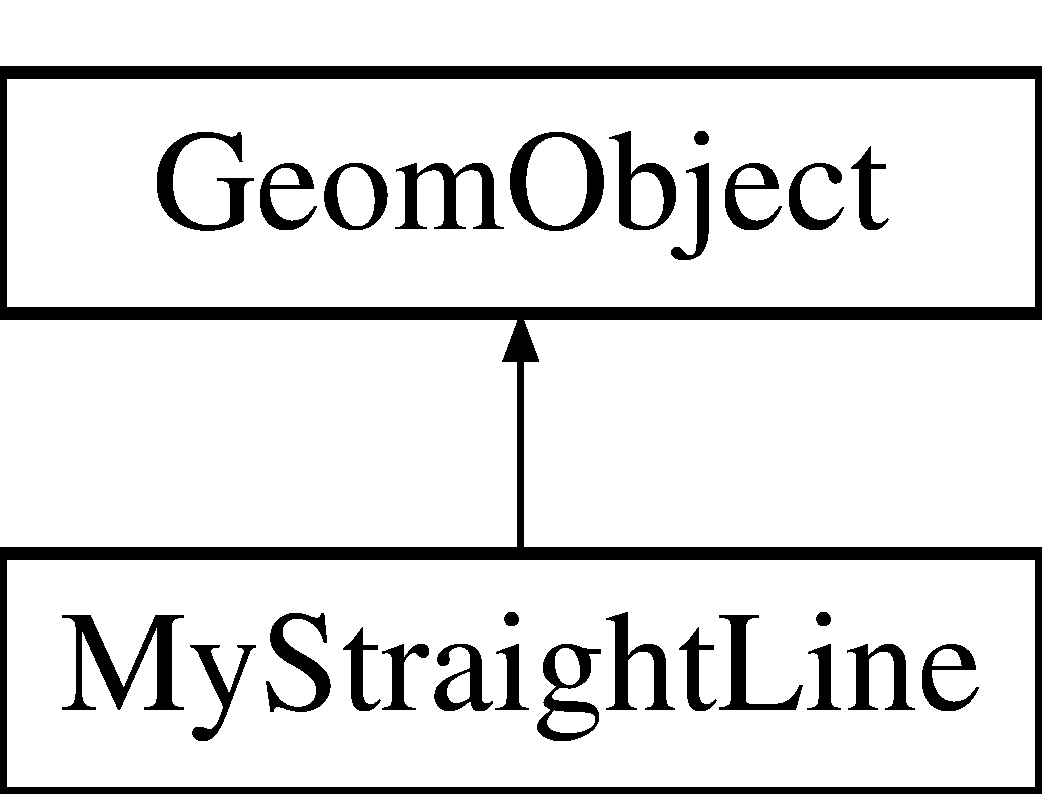
\includegraphics[height=2.000000cm]{classMyStraightLine}
\end{center}
\end{figure}
\subsection*{Public Member Functions}
\begin{DoxyCompactItemize}
\item 
\hyperlink{classMyStraightLine_a2c63e574f21703250a31fc446ab8045d}{My\+Straight\+Line} (const Vector$<$ double $>$ \&r\+\_\+start, const Vector$<$ double $>$ \&r\+\_\+end)
\begin{DoxyCompactList}\small\item\em Constructor\+: Pass start and end points. \end{DoxyCompactList}\item 
\hyperlink{classMyStraightLine_a4c42312f35a3cf72f2f39e88ad28202f}{My\+Straight\+Line} (const \hyperlink{classMyStraightLine}{My\+Straight\+Line} \&dummy)
\begin{DoxyCompactList}\small\item\em Broken copy constructor. \end{DoxyCompactList}\item 
\hyperlink{classMyStraightLine_ae2f9a5860652a726b2f4dc94d1332ef1}{$\sim$\+My\+Straight\+Line} ()
\begin{DoxyCompactList}\small\item\em Destructor\+: Empty. \end{DoxyCompactList}\item 
void \hyperlink{classMyStraightLine_ae3ee51a7b81acc2ef652bec4ee955d2f}{position} (const Vector$<$ double $>$ \&zeta, Vector$<$ double $>$ \&r) const
\begin{DoxyCompactList}\small\item\em Position Vector at Lagrangian coordinate zeta. \end{DoxyCompactList}\end{DoxyCompactItemize}
\subsection*{Private Attributes}
\begin{DoxyCompactItemize}
\item 
Vector$<$ double $>$ \hyperlink{classMyStraightLine_a0f66636dd5d1e7ff6ec93acf90879f0c}{R\+\_\+start}
\begin{DoxyCompactList}\small\item\em Start point of line. \end{DoxyCompactList}\item 
Vector$<$ double $>$ \hyperlink{classMyStraightLine_afa466e12301ccea99a02fe1bde615691}{R\+\_\+end}
\begin{DoxyCompactList}\small\item\em End point of line. \end{DoxyCompactList}\end{DoxyCompactItemize}


\subsection{Detailed Description}
Straight 1D line in 2D space. 

Definition at line 68 of file unstructured\+\_\+fourier\+\_\+decomposed\+\_\+acoustic\+\_\+fsi.\+cc.



\subsection{Constructor \& Destructor Documentation}
\mbox{\Hypertarget{classMyStraightLine_a2c63e574f21703250a31fc446ab8045d}\label{classMyStraightLine_a2c63e574f21703250a31fc446ab8045d}} 
\index{My\+Straight\+Line@{My\+Straight\+Line}!My\+Straight\+Line@{My\+Straight\+Line}}
\index{My\+Straight\+Line@{My\+Straight\+Line}!My\+Straight\+Line@{My\+Straight\+Line}}
\subsubsection{\texorpdfstring{My\+Straight\+Line()}{MyStraightLine()}\hspace{0.1cm}{\footnotesize\ttfamily [1/2]}}
{\footnotesize\ttfamily My\+Straight\+Line\+::\+My\+Straight\+Line (\begin{DoxyParamCaption}\item[{const Vector$<$ double $>$ \&}]{r\+\_\+start,  }\item[{const Vector$<$ double $>$ \&}]{r\+\_\+end }\end{DoxyParamCaption})\hspace{0.3cm}{\ttfamily [inline]}}



Constructor\+: Pass start and end points. 



Definition at line 74 of file unstructured\+\_\+fourier\+\_\+decomposed\+\_\+acoustic\+\_\+fsi.\+cc.

\mbox{\Hypertarget{classMyStraightLine_a4c42312f35a3cf72f2f39e88ad28202f}\label{classMyStraightLine_a4c42312f35a3cf72f2f39e88ad28202f}} 
\index{My\+Straight\+Line@{My\+Straight\+Line}!My\+Straight\+Line@{My\+Straight\+Line}}
\index{My\+Straight\+Line@{My\+Straight\+Line}!My\+Straight\+Line@{My\+Straight\+Line}}
\subsubsection{\texorpdfstring{My\+Straight\+Line()}{MyStraightLine()}\hspace{0.1cm}{\footnotesize\ttfamily [2/2]}}
{\footnotesize\ttfamily My\+Straight\+Line\+::\+My\+Straight\+Line (\begin{DoxyParamCaption}\item[{const \hyperlink{classMyStraightLine}{My\+Straight\+Line} \&}]{dummy }\end{DoxyParamCaption})\hspace{0.3cm}{\ttfamily [inline]}}



Broken copy constructor. 



Definition at line 80 of file unstructured\+\_\+fourier\+\_\+decomposed\+\_\+acoustic\+\_\+fsi.\+cc.

\mbox{\Hypertarget{classMyStraightLine_ae2f9a5860652a726b2f4dc94d1332ef1}\label{classMyStraightLine_ae2f9a5860652a726b2f4dc94d1332ef1}} 
\index{My\+Straight\+Line@{My\+Straight\+Line}!````~My\+Straight\+Line@{$\sim$\+My\+Straight\+Line}}
\index{````~My\+Straight\+Line@{$\sim$\+My\+Straight\+Line}!My\+Straight\+Line@{My\+Straight\+Line}}
\subsubsection{\texorpdfstring{$\sim$\+My\+Straight\+Line()}{~MyStraightLine()}}
{\footnotesize\ttfamily My\+Straight\+Line\+::$\sim$\+My\+Straight\+Line (\begin{DoxyParamCaption}{ }\end{DoxyParamCaption})\hspace{0.3cm}{\ttfamily [inline]}}



Destructor\+: Empty. 



Definition at line 86 of file unstructured\+\_\+fourier\+\_\+decomposed\+\_\+acoustic\+\_\+fsi.\+cc.



\subsection{Member Function Documentation}
\mbox{\Hypertarget{classMyStraightLine_ae3ee51a7b81acc2ef652bec4ee955d2f}\label{classMyStraightLine_ae3ee51a7b81acc2ef652bec4ee955d2f}} 
\index{My\+Straight\+Line@{My\+Straight\+Line}!position@{position}}
\index{position@{position}!My\+Straight\+Line@{My\+Straight\+Line}}
\subsubsection{\texorpdfstring{position()}{position()}}
{\footnotesize\ttfamily void My\+Straight\+Line\+::position (\begin{DoxyParamCaption}\item[{const Vector$<$ double $>$ \&}]{zeta,  }\item[{Vector$<$ double $>$ \&}]{r }\end{DoxyParamCaption}) const\hspace{0.3cm}{\ttfamily [inline]}}



Position Vector at Lagrangian coordinate zeta. 



Definition at line 89 of file unstructured\+\_\+fourier\+\_\+decomposed\+\_\+acoustic\+\_\+fsi.\+cc.



\subsection{Member Data Documentation}
\mbox{\Hypertarget{classMyStraightLine_afa466e12301ccea99a02fe1bde615691}\label{classMyStraightLine_afa466e12301ccea99a02fe1bde615691}} 
\index{My\+Straight\+Line@{My\+Straight\+Line}!R\+\_\+end@{R\+\_\+end}}
\index{R\+\_\+end@{R\+\_\+end}!My\+Straight\+Line@{My\+Straight\+Line}}
\subsubsection{\texorpdfstring{R\+\_\+end}{R\_end}}
{\footnotesize\ttfamily Vector$<$double$>$ My\+Straight\+Line\+::\+R\+\_\+end\hspace{0.3cm}{\ttfamily [private]}}



End point of line. 



Definition at line 102 of file unstructured\+\_\+fourier\+\_\+decomposed\+\_\+acoustic\+\_\+fsi.\+cc.

\mbox{\Hypertarget{classMyStraightLine_a0f66636dd5d1e7ff6ec93acf90879f0c}\label{classMyStraightLine_a0f66636dd5d1e7ff6ec93acf90879f0c}} 
\index{My\+Straight\+Line@{My\+Straight\+Line}!R\+\_\+start@{R\+\_\+start}}
\index{R\+\_\+start@{R\+\_\+start}!My\+Straight\+Line@{My\+Straight\+Line}}
\subsubsection{\texorpdfstring{R\+\_\+start}{R\_start}}
{\footnotesize\ttfamily Vector$<$double$>$ My\+Straight\+Line\+::\+R\+\_\+start\hspace{0.3cm}{\ttfamily [private]}}



Start point of line. 



Definition at line 99 of file unstructured\+\_\+fourier\+\_\+decomposed\+\_\+acoustic\+\_\+fsi.\+cc.



The documentation for this class was generated from the following file\+:\begin{DoxyCompactItemize}
\item 
\hyperlink{unstructured__fourier__decomposed__acoustic__fsi_8cc}{unstructured\+\_\+fourier\+\_\+decomposed\+\_\+acoustic\+\_\+fsi.\+cc}\end{DoxyCompactItemize}

\chapter{File Documentation}
\hypertarget{acoustic__fsi_8cc}{}\section{acoustic\+\_\+fsi.\+cc File Reference}
\label{acoustic__fsi_8cc}\index{acoustic\+\_\+fsi.\+cc@{acoustic\+\_\+fsi.\+cc}}
\subsection*{Classes}
\begin{DoxyCompactItemize}
\item 
class \hyperlink{classCoatedDiskProblem}{Coated\+Disk\+Problem$<$ E\+L\+A\+S\+T\+I\+C\+I\+T\+Y\+\_\+\+E\+L\+E\+M\+E\+N\+T, H\+E\+L\+M\+H\+O\+L\+T\+Z\+\_\+\+E\+L\+E\+M\+E\+N\+T $>$}
\begin{DoxyCompactList}\small\item\em Coated disk F\+SI. \end{DoxyCompactList}\end{DoxyCompactItemize}
\subsection*{Namespaces}
\begin{DoxyCompactItemize}
\item 
 \hyperlink{namespaceGlobal__Parameters}{Global\+\_\+\+Parameters}
\begin{DoxyCompactList}\small\item\em Global variables. \end{DoxyCompactList}\end{DoxyCompactItemize}
\subsection*{Functions}
\begin{DoxyCompactItemize}
\item 
Time\+Harmonic\+Isotropic\+Elasticity\+Tensor \hyperlink{namespaceGlobal__Parameters_aeeb26e11ef275bdfce14710e00290bb6}{Global\+\_\+\+Parameters\+::E} (Nu)
\begin{DoxyCompactList}\small\item\em The elasticity tensor for the solid. \end{DoxyCompactList}\item 
void \hyperlink{namespaceGlobal__Parameters_ae0f9a80fb7510dbfbbef22582da231b7}{Global\+\_\+\+Parameters\+::update\+\_\+parameter\+\_\+values} ()
\begin{DoxyCompactList}\small\item\em Function to update dependent parameter values. \end{DoxyCompactList}\item 
void \hyperlink{namespaceGlobal__Parameters_ab51fa55d06d9963d363bcf966cfcc62b}{Global\+\_\+\+Parameters\+::solid\+\_\+boundary\+\_\+displacement} (const Vector$<$ double $>$ \&x, Vector$<$ std\+::complex$<$ double $>$ $>$ \&u)
\begin{DoxyCompactList}\small\item\em Displacement field on inner boundary of solid. \end{DoxyCompactList}\item 
std\+::complex$<$ double $>$ \hyperlink{namespaceGlobal__Parameters_a116765fbd117ec6199c9399af801d510}{Global\+\_\+\+Parameters\+::\+Hankel\+H1} (const double \&k, const double \&x)
\begin{DoxyCompactList}\small\item\em Interface to Hankel function in maple style. \end{DoxyCompactList}\item 
std\+::complex$<$ double $>$ \hyperlink{namespaceGlobal__Parameters_a12dd327bc592b36ffd4abbab5018146f}{Global\+\_\+\+Parameters\+::axisym\+\_\+coefficient} ()
\begin{DoxyCompactList}\small\item\em Coefficient in front of Hankel function for axisymmetric solution of Helmholtz potential. \end{DoxyCompactList}\item 
void \hyperlink{namespaceGlobal__Parameters_af95baf4096a1393ab06bfa9ff9a57a35}{Global\+\_\+\+Parameters\+::exact\+\_\+axisym\+\_\+potential} (const Vector$<$ double $>$ \&x, Vector$<$ double $>$ \&soln)
\begin{DoxyCompactList}\small\item\em Exact solution for Helmholtz potential for axisymmetric solution. \end{DoxyCompactList}\item 
double \hyperlink{namespaceGlobal__Parameters_a79131fd1bf3eb1ab080c21c2d98a92d5}{Global\+\_\+\+Parameters\+::exact\+\_\+axisym\+\_\+radiated\+\_\+power} ()
\begin{DoxyCompactList}\small\item\em Exact radiated power for axisymmetric solution. \end{DoxyCompactList}\item 
int \hyperlink{acoustic__fsi_8cc_a3c04138a5bfe5d72780bb7e82a18e627}{main} (int argc, char $\ast$$\ast$argv)
\begin{DoxyCompactList}\small\item\em Driver for acoustic fsi problem. \end{DoxyCompactList}\end{DoxyCompactItemize}
\subsection*{Variables}
\begin{DoxyCompactItemize}
\item 
double \hyperlink{namespaceGlobal__Parameters_a91a3fa265abaf9e724c668ee800ffb29}{Global\+\_\+\+Parameters\+::\+K\+\_\+squared} =10.\+0
\begin{DoxyCompactList}\small\item\em Square of wavenumber for the Helmholtz equation. \end{DoxyCompactList}\item 
double \hyperlink{namespaceGlobal__Parameters_a88ded445ecd7bd89701409e68fd0b900}{Global\+\_\+\+Parameters\+::\+Outer\+\_\+radius} =4.\+0
\begin{DoxyCompactList}\small\item\em Radius of outer boundary of Helmholtz domain. \end{DoxyCompactList}\item 
double \hyperlink{namespaceGlobal__Parameters_a7814fddf663e56168174a42d2cd6b4c1}{Global\+\_\+\+Parameters\+::Q} =0.\+0
\begin{DoxyCompactList}\small\item\em F\+SI parameter. \end{DoxyCompactList}\item 
double \hyperlink{namespaceGlobal__Parameters_ae3cf8878ede839bffda01f79bbe3e819}{Global\+\_\+\+Parameters\+::\+H\+\_\+coating} =0.\+3
\begin{DoxyCompactList}\small\item\em Non-\/dim thickness of elastic coating. \end{DoxyCompactList}\item 
double \hyperlink{namespaceGlobal__Parameters_a20fccdcfa2c15ad8b951b9ada3bb1661}{Global\+\_\+\+Parameters\+::\+Nu} = 0.\+3
\begin{DoxyCompactList}\small\item\em Poisson\textquotesingle{}s ratio. \end{DoxyCompactList}\item 
double \hyperlink{namespaceGlobal__Parameters_a517d4c31b8bce6563c2f605266dd9679}{Global\+\_\+\+Parameters\+::\+Density\+\_\+ratio} =0.\+0
\begin{DoxyCompactList}\small\item\em Density ratio\+: solid to fluid. \end{DoxyCompactList}\item 
double \hyperlink{namespaceGlobal__Parameters_af9e1e178dfb7f5e35b452599bd4c4324}{Global\+\_\+\+Parameters\+::\+Omega\+\_\+sq} =0.\+0
\begin{DoxyCompactList}\small\item\em Non-\/dim square of frequency for solid -- dependent variable! \end{DoxyCompactList}\item 
unsigned \hyperlink{namespaceGlobal__Parameters_aff31353c09f439f3d537ad06ce868787}{Global\+\_\+\+Parameters\+::N} =0
\begin{DoxyCompactList}\small\item\em Azimuthal wavenumber for imposed displacement of coating on inner boundary. \end{DoxyCompactList}\item 
string \hyperlink{namespaceGlobal__Parameters_a301ab922df72030c660b21328d6caf76}{Global\+\_\+\+Parameters\+::\+Directory} =\char`\"{}R\+E\+S\+LT\char`\"{}
\begin{DoxyCompactList}\small\item\em Output directory. \end{DoxyCompactList}\item 
unsigned \hyperlink{namespaceGlobal__Parameters_a35d5d2ecfff0cec6150a5dc79e5c1ad1}{Global\+\_\+\+Parameters\+::\+El\+\_\+multiplier} =1
\begin{DoxyCompactList}\small\item\em Multiplier for number of elements. \end{DoxyCompactList}\end{DoxyCompactItemize}


\subsection{Function Documentation}
\mbox{\Hypertarget{acoustic__fsi_8cc_a3c04138a5bfe5d72780bb7e82a18e627}\label{acoustic__fsi_8cc_a3c04138a5bfe5d72780bb7e82a18e627}} 
\index{acoustic\+\_\+fsi.\+cc@{acoustic\+\_\+fsi.\+cc}!main@{main}}
\index{main@{main}!acoustic\+\_\+fsi.\+cc@{acoustic\+\_\+fsi.\+cc}}
\subsubsection{\texorpdfstring{main()}{main()}}
{\footnotesize\ttfamily int main (\begin{DoxyParamCaption}\item[{int}]{argc,  }\item[{char $\ast$$\ast$}]{argv }\end{DoxyParamCaption})}



Driver for acoustic fsi problem. 



Definition at line 849 of file acoustic\+\_\+fsi.\+cc.



References Global\+\_\+\+Parameters\+::\+Directory, Coated\+Disk\+Problem$<$ E\+L\+A\+S\+T\+I\+C\+I\+T\+Y\+\_\+\+E\+L\+E\+M\+E\+N\+T, H\+E\+L\+M\+H\+O\+L\+T\+Z\+\_\+\+E\+L\+E\+M\+E\+N\+T $>$\+::doc\+\_\+solution(), Global\+\_\+\+Parameters\+::\+El\+\_\+multiplier, Global\+\_\+\+Parameters\+::N, Global\+\_\+\+Parameters\+::\+Outer\+\_\+radius, Global\+\_\+\+Parameters\+::Q, and Global\+\_\+\+Parameters\+::update\+\_\+parameter\+\_\+values().


\hypertarget{acoustic__fsi__annulus_8txt__doxygenified_8h}{}\section{acoustic\+\_\+fsi\+\_\+annulus.\+txt\+\_\+doxygenified.\+h File Reference}
\label{acoustic__fsi__annulus_8txt__doxygenified_8h}\index{acoustic\+\_\+fsi\+\_\+annulus.\+txt\+\_\+doxygenified.\+h@{acoustic\+\_\+fsi\+\_\+annulus.\+txt\+\_\+doxygenified.\+h}}

\hypertarget{unstructured__acoustic__fsi_8cc}{}\section{unstructured\+\_\+acoustic\+\_\+fsi.\+cc File Reference}
\label{unstructured__acoustic__fsi_8cc}\index{unstructured\+\_\+acoustic\+\_\+fsi.\+cc@{unstructured\+\_\+acoustic\+\_\+fsi.\+cc}}
\subsection*{Classes}
\begin{DoxyCompactItemize}
\item 
class \hyperlink{classMyStraightLine}{My\+Straight\+Line}
\begin{DoxyCompactList}\small\item\em Straight 1D line in 2D space. \end{DoxyCompactList}\item 
class \hyperlink{classCoatedDiskProblem}{Coated\+Disk\+Problem$<$ E\+L\+A\+S\+T\+I\+C\+I\+T\+Y\+\_\+\+E\+L\+E\+M\+E\+N\+T, H\+E\+L\+M\+H\+O\+L\+T\+Z\+\_\+\+E\+L\+E\+M\+E\+N\+T $>$}
\begin{DoxyCompactList}\small\item\em Coated disk F\+SI. \end{DoxyCompactList}\end{DoxyCompactItemize}
\subsection*{Namespaces}
\begin{DoxyCompactItemize}
\item 
 \hyperlink{namespaceGlobal__Parameters}{Global\+\_\+\+Parameters}
\begin{DoxyCompactList}\small\item\em Global variables. \end{DoxyCompactList}\end{DoxyCompactItemize}
\subsection*{Functions}
\begin{DoxyCompactItemize}
\item 
Vector$<$ double $>$ \hyperlink{namespaceGlobal__Parameters_a461bb148c1f6494672520bdf8045483f}{Global\+\_\+\+Parameters\+::\+Omega\+\_\+sq} (2, 0.\+0)
\begin{DoxyCompactList}\small\item\em Square of non-\/dim frequency for the two regions -- dependent variable! \end{DoxyCompactList}\item 
Vector$<$ double $>$ \hyperlink{namespaceGlobal__Parameters_a3ad42a80620a3847cf0d1b187e2ed2ec}{Global\+\_\+\+Parameters\+::\+Density\+\_\+ratio} (2, 0.\+1)
\begin{DoxyCompactList}\small\item\em Density ratio for the two regions\+: solid to fluid. \end{DoxyCompactList}\item 
void \hyperlink{namespaceGlobal__Parameters_ae0f9a80fb7510dbfbbef22582da231b7}{Global\+\_\+\+Parameters\+::update\+\_\+parameter\+\_\+values} ()
\begin{DoxyCompactList}\small\item\em Function to update dependent parameter values. \end{DoxyCompactList}\item 
void \hyperlink{namespaceGlobal__Parameters_a0ddb3a77481b907fbb34f2e8d0a6eb9f}{Global\+\_\+\+Parameters\+::pressure\+\_\+load} (const Vector$<$ double $>$ \&x, const Vector$<$ double $>$ \&n, Vector$<$ std\+::complex$<$ double $>$ $>$ \&traction)
\begin{DoxyCompactList}\small\item\em Pressure load (real and imag part) \end{DoxyCompactList}\item 
int \hyperlink{unstructured__acoustic__fsi_8cc_a3c04138a5bfe5d72780bb7e82a18e627}{main} (int argc, char $\ast$$\ast$argv)
\begin{DoxyCompactList}\small\item\em Driver for acoustic fsi problem. \end{DoxyCompactList}\end{DoxyCompactItemize}
\subsection*{Variables}
\begin{DoxyCompactItemize}
\item 
unsigned \hyperlink{namespaceGlobal__Parameters_ae16eb10039cab2098b02ec7dff946277}{Global\+\_\+\+Parameters\+::\+A\+B\+C\+\_\+order} =3
\begin{DoxyCompactList}\small\item\em Order of absorbing/appproximate boundary condition. \end{DoxyCompactList}\item 
Vector$<$ Time\+Harmonic\+Isotropic\+Elasticity\+Tensor $\ast$ $>$ \hyperlink{namespaceGlobal__Parameters_a73c731fa617a9d92851e4195493262e7}{Global\+\_\+\+Parameters\+::\+E\+\_\+pt}
\begin{DoxyCompactList}\small\item\em The elasticity tensors for the two regions. \end{DoxyCompactList}\item 
double \hyperlink{namespaceGlobal__Parameters_a31fb55c20db4aa0127aafa20f0d76731}{Global\+\_\+\+Parameters\+::P} = 0.\+1
\begin{DoxyCompactList}\small\item\em Uniform pressure. \end{DoxyCompactList}\item 
double \hyperlink{namespaceGlobal__Parameters_afbe27ad463a1fb23cb99d029a9fac731}{Global\+\_\+\+Parameters\+::\+Alpha} =200.\+0
\begin{DoxyCompactList}\small\item\em Peakiness parameter for pressure load. \end{DoxyCompactList}\end{DoxyCompactItemize}


\subsection{Function Documentation}
\mbox{\Hypertarget{unstructured__acoustic__fsi_8cc_a3c04138a5bfe5d72780bb7e82a18e627}\label{unstructured__acoustic__fsi_8cc_a3c04138a5bfe5d72780bb7e82a18e627}} 
\index{unstructured\+\_\+acoustic\+\_\+fsi.\+cc@{unstructured\+\_\+acoustic\+\_\+fsi.\+cc}!main@{main}}
\index{main@{main}!unstructured\+\_\+acoustic\+\_\+fsi.\+cc@{unstructured\+\_\+acoustic\+\_\+fsi.\+cc}}
\subsubsection{\texorpdfstring{main()}{main()}}
{\footnotesize\ttfamily int main (\begin{DoxyParamCaption}\item[{int}]{argc,  }\item[{char $\ast$$\ast$}]{argv }\end{DoxyParamCaption})}



Driver for acoustic fsi problem. 



Definition at line 1260 of file unstructured\+\_\+acoustic\+\_\+fsi.\+cc.



References Global\+\_\+\+Parameters\+::\+Alpha, Global\+\_\+\+Parameters\+::\+Density\+\_\+ratio, Global\+\_\+\+Parameters\+::\+Directory, Global\+\_\+\+Parameters\+::\+E\+\_\+pt, Global\+\_\+\+Parameters\+::\+El\+\_\+multiplier, Global\+\_\+\+Parameters\+::\+Nu, Global\+\_\+\+Parameters\+::\+Outer\+\_\+radius, Global\+\_\+\+Parameters\+::Q, and Global\+\_\+\+Parameters\+::update\+\_\+parameter\+\_\+values().


%--- End generated contents ---

% Index
\backmatter
\newpage
\phantomsection
\clearemptydoublepage
\addcontentsline{toc}{chapter}{Index}
\printindex

\end{document}
